\chapter{MDL}
\label{chap:MGS-MDL}

MGS is composed of 2 parts
\begin{enumerate}
  \item MDL : the script that helps generating C++ classes that conform to MGS
  code standard (Chap.\ref{chap:MGS-MDL})
  
  \item GSL : the script that helps to connect different C++ classes together in
  a graph-based simulator system. (Chap.\ref{chap:MGS-GSL}) 
\end{enumerate}

\section{MDF}
\label{sec:MDF}

We can generate code for a new MGS component using \verb!mdlparser! with the
given *.mdl file (Sect.\ref{sec:MDL}). To help generating MGS components from
multiple *.mdl files, we can put them into a single *.mdf file, and run
\verb!./define! script.

An *.mdf file is used to include many *.mdl files (Sect.\ref{sec:MDL-script})
together. 
\begin{verbatim}
../gsl/extensions/functor/functors.mdf

../gsl/extensions/struct/structs.mdf
   #include "CoordsStruct.mdl"    
../gsl/extensions/variable/variables.mdf
../models/compartmental.mdf
\end{verbatim}

Example: we can use the script \verb!./define!
\begin{verbatim}
./define compartment.mdf
\end{verbatim}
which run throughs all *.mdl files inside the compartment.mdf file, and
parse them using \verb!mdlparser! (Sect.\ref{sec:mdlparser}).

\subsection{define script}

{\tiny
\begin{verbatim}
#!/bin/bash

sed '/\\/p' $1 | sed 's/#include "/cd /g' | sed 's/\// ; $MDLROOT\/bin\/mdlparser /g' | sed 's/"/ ; sh copyModules ; cd .. ;/g' > defineModels1.sh;
awk '{ print "if [ '$1' -ot " $2 "/" $5 " ] || [ define -ot '$1' ]; then " $0 " fi" }' defineModels1.sh > defineModels2.sh;
source defineModels2.sh;
touch $1;
rm -f defineModels1.sh;
rm -f defineModels2.sh;
if grep include $1; then $MDLROOT/bin/mdlparser $1 -i $LENSROOT/extensions/variable:$LENSROOT/extensions/struct; fi
touch define;
\end{verbatim}
}

\subsection{functors.mdf}
\label{sec:functors.mdf}

Example: functors.mdf
\begin{verbatim}
#include "BinomialDist.mdl"                                                                                                                                                                            
#include "CombineNVPairs.mdl"
#include "ConnectNodeSetsFunctor.mdl"
#include "DstDimensionConstrainedSampler.mdl"
#include "DstRefDistanceModifier.mdl"
#include "DstRefGaussianWeightModifier.mdl"
#include "DstRefSumRsqrdInvWeightModifier.mdl"
#include "DstScaledContractedGaussianWeightModifier.mdl"
#include "DstScaledGaussianWeightModifier.mdl"
#include "GetDstNodeCoordFunctor.mdl"
#include "GetNodeCoordFunctor.mdl"
#include "GetPreNodeCoordFunctor.mdl"
#include "GetPreNodeIndex.mdl"
#include "GetPostNodeCoordFunctor.mdl"
#include "IsoSampler.mdl"
#include "ModifyParameterSet.mdl"
#include "NameReturnValue.mdl"
#include "PolyConnectorFunctor.mdl"
#include "RefAngleModifier.mdl"
#include "RefDistanceModifier.mdl"
#include "ReversedDstRefGaussianWeightModifier.mdl"
#include "ReversedSrcRefGaussianWeightModifier.mdl" 
#include "ReverseFunctor.mdl"
#include "ServiceConnectorFunctor.mdl"
#include "SrcDimensionConstrainedSampler.mdl"
#include "SrcRefDistanceModifier.mdl"
#include "SrcRefGaussianWeightModifier.mdl"
#include "SrcRefPeakedWeightModifier.mdl"
#include "SrcRefSumRsqrdInvWeightModifier.mdl"
#include "SrcScaledContractedGaussianWeightModifier.mdl"
#include "SrcScaledGaussianWeightModifier.mdl"
#include "ToroidalRadialSampler.mdl"
#include "TissueConnectorFunctor.mdl"
#include "TissueFunctor.mdl"
#include "TissueLayoutFunctor.mdl"
#include "TissueNodeInitFunctor.mdl"
#include "TissueProbeFunctor.mdl"
#include "UniformDiscreteDist.mdl"
\end{verbatim}



\subsection{compartments.mdf}

NOTE: \verb!./make_nts! makes call automatically
\begin{verbatim}
./define compartmental.mdf
\end{verbatim}


Example: compartments.mdf
\begin{verbatim}
#include "std/std.mdl"                                                                                                                                                                                 
#include "LaboratoryTools/LaboratoryTools.mdl"
#include "BranchSolver/BranchSolver.mdl"
#include "HodgkinHuxley/HodgkinHuxley.mdl"
#include "HodgkinHuxleyVoltage/HodgkinHuxleyVoltage.mdl"
#include "HodgkinHuxleyVoltageJunction/HodgkinHuxleyVoltageJunction.mdl"
#include "NaChannel/NaChannel.mdl"
#include "NaChannel_AIS/NaChannel_AIS.mdl"
#include "KDRChannel/KDRChannel.mdl"
#include "KDRChannel_AIS/KDRChannel_AIS.mdl"
#include "KDRChannel_IO/KDRChannel_IO.mdl"
#include "Connexon/Connexon.mdl"
#include "PreSynapticPoint/PreSynapticPoint.mdl"
#include "GABAAReceptor/GABAAReceptor.mdl"
#include "AMPAReceptor/AMPAReceptor.mdl"
#include "CaConcentration/CaConcentration.mdl"
#include "CaConcentrationJunction/CaConcentrationJunction.mdl"
#include "CahChannel/CahChannel.mdl"
#include "CalChannel/CalChannel.mdl"
#include "KCaChannel/KCaChannel.mdl"
#include "HCNChannel/HCNChannel.mdl"
#include "CaConnexon/CaConnexon.mdl"
#include "NMDAReceptor/NMDAReceptor.mdl"
#include "ChannelHayNat/ChannelHayNat.mdl"
#include "ChannelHayNap/ChannelHayNap.mdl"
#include "ChannelHayHCN/ChannelHayHCN.mdl"
#include "ChannelHayMK/ChannelHayMK.mdl"
#include "ChannelHayKp/ChannelHayKp.mdl"
#include "ChannelHayKt/ChannelHayKt.mdl"
#include "ChannelHayKv31/ChannelHayKv31.mdl"
#include "ChannelHayCaHVA/ChannelHayCaHVA.mdl"
#include "ChannelHayCaLVA/ChannelHayCaLVA.mdl"
#include "ChannelHaySK/ChannelHaySK.mdl"
#include "ChannelHodgkinKDR/ChannelHodgkinKDR.mdl"
#include "ChannelHodgkinNat/ChannelHodgkinNat.mdl"
#include "ChannelSchweighoferCah/ChannelSchweighoferCah.mdl"
#include "ChannelSchweighoferCal/ChannelSchweighoferCal.mdl"
#include "ChannelSchweighoferHCN/ChannelSchweighoferHCN.mdl"
#include "ChannelSchweighoferKCa/ChannelSchweighoferKCa.mdl"
#include "ChannelSchweighoferKDR/ChannelSchweighoferKDR.mdl"
#include "ChannelSchweighoferNat/ChannelSchweighoferNat.mdl"
\end{verbatim}

\section{MDL mdlparser: main() - How it works}
\label{sec:MDL}
\label{sec:mdlparser}
\label{sec:mdl.tab.c}
\label{sec:Initializer-mdlparser}


MDL helps generating code that facilitate the interface between different
components to be managed by the MGS framework, the details of the behavior of
these components need to be implemented by user (check Step 4).

Once the user run 
\begin{verbatim}
mdlparser File.mdl
\end{verbatim}
the binary \verb!mdlparser! will read the content of the file and perform the
below steps.

The \verb!main()! function of \verb!mdlparser! is in 
\verb!./mdl/parser/mdl.y! file (which is generated into mdl.tab.c file)
\begin{lstlisting}
void main(int argc, char** argv)
{
   Initializer init(argc, argv);
   if (init.execute()) {
      return 0;
   } else {
      return 1;
   }
}
\end{lstlisting}

To parse MDL script, we define MdlLexer class (Sect.\ref{sec:MdlLexer-class});
and to parser GSL script, we use LensLexer class (Sect.\ref{sec:LensLexer}).

\subsection{MdlLexer: parsing MDL script, and generate C++ files}
\label{sec:MdlLexer-class}

First, your parser need to be derived from \verb!yyFlexLexer! class, i.e. in the
*.l file
\begin{verbatim}
%option c++
%option yyclass="MdlLexer"
\end{verbatim} 

WHOLE PROCESS:
\begin{verbatim}
scanner.reset(new MdlLexer(infile, outfile));
context.reset(new MdlContext());

context._lexer = scanner.get() ; //read the input script file
_generatables = new MemberContainer<Generatable>();

context->_generatables = _generatables;

mdlparse(context.get()); //parse it, and update context->_generatables
   // a _generatables[i] hold a single construct, e.g. a Node definition, 
   // Struct definition

MemberContainer<Generatable>::const_iterator end =
           context->_generatables->end();

for (it = context->_generatables->begin(); it != end; ++it)
{
// depending on the runtime type of 'Generatable*', e.g.
//   InterfaceImplementorBase, or 
  it->second->generate();  //spit out the C++ generated code to standard std::cout
                    //with some modification to data type, such as int*[] 
                    // (an array) is turned into
                    //  ShallowArray<int*>
}

for (it = context->_generatables->begin(); it != end; ++it)
{
  it->second->generateFiles(fileName);  //spit out the C++ generated code to
                                       //files and folder
                         // check Generatable::
}
\end{verbatim}

Whenever mdlparser (Sect.\ref{sec:mdlparser}) execute a statement read-in from
the GSL script, all information required are stored in the so-called context.


To understand the parsing process, please read Sect.\ref{sec:C_production-MDL}
that describes \verb!C_production! class and its derivatives.
Each time the context object's \verb!execute()! method is called; it goes
through all statements (as an object of derived class of \verb!C_production!
class in the MDL script, and store all information as read-in into properly
structure into the derived class of \verb!C_production! class.

\begin{enumerate}
  \item \verb!C_node!: what matters is that the \verb!execute()! calls 
  
Suppose \verb!Node LifeNode! is detected, its then create the interfaces 
(by calling executeInterfaceImplementorBase - Sect.\ref{sec:InterfaceImplementorBase::getAddConnectionFunctionBody()}),
create the \verb!CG_LifeNodeCompCategory! class (by calling executeCompCategoryBase()), \ldots
finally add that to the generatable-list (Sect.\ref{sec:Generatable-class}).

\begin{verbatim}
C_node::execute(...)
{
  Node* cc = new Node(getFileName());
   executeInterfaceImplementorBase(context, cc);
   executeCompCategoryBase(context, cc);
   executeSharedCCBase(context, cc);
   executeConnectionCCBase(context, cc);
   cc->checkAllMemberToInterfaces();

   std::auto_ptr<Generatable> nodeMember;
   nodeMember.reset(cc);
   context->_generatables->addMember(_name, nodeMember);
}
\end{verbatim}


NOTE:
\begin{verbatim}
// C_shared'CompCategory'Base
class C_node: public C_sharedCCBase {
  virtual void execute(...);

}

class C_sharedCCBase: public C_connectionCCBase{
  virtual void execute(...);
  void executeSharedCCBase(...);

}

class C_connectionCCBase: public C_compCategoryBase {
  virtual void execute(...);
  void executeConnectionCCBase(...);

}

class C_compCategoryBase: public C_interfaceImplementorBase {
  virtual void execute(...);
  void executeCompCategoryBase(...);
}

class C_interfaceImplementorBase: public C_production {

  virtual void executeInterfaceImplementorBase(...);
  
protected:
  std::string _name;
  C_interfacePointerList* _interfacePointerList;
  C_generalList* _generalList;
}
\end{verbatim}

  \item \verb!C_edge! 
\end{enumerate}

The parser makes use of the following classes, depending upon the kind of construct that it parses


\subsection{-- loop 1}


This loops does some processing and spit MDL to standard output
\begin{verbatim}
for (it = context->_generatables->begin(); it != end; ++it)
{
// depending on the runtime type of 'Generatable*', e.g. InterfaceImplementorBase, or 
  it->second->generate();  //spit out the C++ generated code to standard std::cout
                    //with some modification to data type, such as int*[] 
                    // (an array) is turned into
                    //  ShallowArray<int*>
}
\end{verbatim}
 
\subsection{-- loop 2}

This loops does generate C++ file, do copy to target location, and generate Extentions.mk if needed.
\begin{verbatim}
for (it = context->_generatables->begin(); it != end; ++it)
{
  it->second->generateFiles(fileName);  //spit out the C++ generated code to
                                       //files and folder
                         // check Generatable::
}
\end{verbatim}


The key method that generate C++ files is
\textcolor{red}{Generatable::generateFiles()} -
Sect.\ref{sec:Generatable-class}.

\subsection{How to code/compile}


In \verb!Makefile! file:
\begin{itemize}
  \item \verb!./mdl/sources.mk! is used by the Makefile file for \verb!make! utility to
figure out source files needed to include in the build.

After that, it builds the dependency files using the depend.sh script.

  \item \verb!./mdl/scripts/depend.sh! script is used to  help building the
 dependency files. 
 
 These dependency files are put into \verb!./obj! directory.
 
 \item The \verb!default! target builds the parser executable.
\begin{verbatim}
default: all

all: $(BASE_OBJECTS) $(LENS_LIBS_EXT) bin/gslparser \
     $(DCA_OBJ)/socket.o $(OBJS)  $(MODULE_MKS)  
\end{verbatim} 
\end{itemize}


\section{Reading in the grammar of MDL}
%\section{MDL framework: C++ class structure}
\label{sec:MDL-code-folder}

\subsection{C\_production (for MDL)}
\label{sec:C_production-MDL}


MGS is a big system that encapsulate everything in a number of base classes, and
provide a tools that enable the generating of new classes derived from these
classes, based on the description (written in .mdl language -
Sect.\ref{sec:MDL-script}) given by the user about the class they want
\verb!mdlparser! to generate.

Similar to the class of the same name being used for gslparser
(Sect.\ref{sec:C_production}), the \verb!C_production! class is the base class
for mdlparser, from that all derived class store all information related to the
construct it reads from MDL script file.

The parser base class is \verb!C_production! which is an abstract class that
define the method (\verb!execute()!) to run once the corresponding token is
recognized inside of which it calls \verb!internalExecute()! function.
During the parsing of the input, i.e. MDL script content, the mdlparser will
call the approriate class to handle the processing.


Every derived class - to handle a particular token - needs to (1) add their own data
member if needed, (2) implement the \verb!internalExecute()! method.
\begin{verbatim}

// representing a construct or a token read-in via MDL file content
class C_production
{
protected:
   int _lineNumber;
   std::string _fileName;

public:
   virtual void execute (MdlContext *);
   // and methods for
   // set/get lineNumber
   // set/get fileName
   // set token location (i.e. fileName + lineNumber
}

\end{verbatim}


The class(es) derived from \verb!C_production! class
\begin{enumerate}
  
  \item \verb!C_interface! class: to handle the processing when an \verb!Interface! declaration is detected from MDL script
  \label{sec:C_interface-MDL}

\begin{verbatim}
Interface ValueProducer{
  int* value;
}
\end{verbatim}  

\begin{lstlisting}
class C_interface: public C_production{
   std::string _name;   // store 'ValueProducer'
   Interface*  _interface; // object to handle the creation of C++ code
   C_dataTypeList*  _dataTypeList; // contains all data members declared for this Interface construct
}
\end{lstlisting}
which then calls \verb!Interface! class (Sect.\ref{sec:Interface-MDL}) to handle the creation of C++ output code.
  
  \item \verb!C_interfaceImplementorBase! class: to handle the processing when an \verb!Implements! declaration is detected from MDL script
  \label{sec:C_interfaceImplementorBase-MDL}

\begin{verbatim}
Node LifeNode Implements ValueProducer{
}
\end{verbatim}
which then calls \verb!InterfaceImplementor! class to handle the creation of C++ output code.


\begin{lstlisting}
class C_interfaceImplementorBase: public C_production {

  executeInterfaceImplementorBase(...);
  
protected:
  std::string _name;  // store 'LifeNode'
  C_interfacePointerList* _interfacePointerList; // the list of all C_interface that this node implements
  C_generalList* _generalList;
}
\end{lstlisting}

 \verb!C_interfaceImplementorBase! is the Bison-based class that calls \verb!InterfaceImplementorBase!
  to handle the creation of output related to Interface - Sect.\ref{sec:InterfaceImplementorBase::getAddConnectionFunctionBody()}
  


   \item \verb!C_generalList!
   
   
   \item \verb!C_general!
\end{enumerate}


\subsection{Initializer::execute()}
\label{sec:Initializer-execute()}

An object  - Sect.\ref{sec:CommandLine-MDL}
\begin{verbatim}
CommandLine  commandline;
\end{verbatim}
just to return the MDL filename to be 

\subsection{Class represent datatype}

\begin{verbatim}
abstract DataType
   |
   LensType
       |
       RepertoireType
       
   
\end{verbatim}

\subsection{DataType}
\label{sec:DataType}

The root class is \verb!DataType!, and provides a number of common classes for
all data types 
\begin{verbatim}

\end{verbatim}
and common data members
\begin{verbatim}
  private:
  std::string getServiceInfoString(const std::string& tab,
                                   const std::string& info) const;

  std::string getOptionalServiceInfoString(const std::string& tab,
                                           const std::string& info) const;

  bool _derived;  // if the data is derived class or 'DataType' class
  bool _shared;  // 
  std::string _name;
  std::string _comment;
  std::vector<std::string> _subAttributePath;
};
\end{verbatim}

\subsection{LensType}
\label{sec:LensType}

\begin{verbatim}
class LensType: public DataType
{

}
\end{verbatim}


\subsection{ServiceType}
\label{sec:ServiceType}

\begin{verbatim}
class ServiceType: public LensType
{

}
\end{verbatim}

\subsection{-- C\_variable}
\label{sec:C_variable}

\begin{lstlisting}
class C_variable: public C_connectionCCBase
{

}
\end{lstlisting}

\subsection{-- C\_connectionCCBase}
\label{sec:C_connectionCCBase}


\subsection{-- C\_compCategoryBase}
\label{sec:C_compCategoryBase}



\subsection{Array: ShallowArray}
\label{sec:Array}

The \verb!ShallowArray! class provides a wrapper to \verb!Array! class, with a
particular initial block size \verb!SUGGESTEDARRAYBLOCKSIZE!, and a particular
incremental step in size \verb!SUGGESTEDBLOCKINCREMENTSIZE! each time.

IMPORTANT:
\begin{itemize}
  \item array is organized as pointers \verb!T** _blocksArray! with T=template
  of any data type
  
\begin{verbatim}
_blocksArray[block_index][index_element_in_block]
\end{verbatim}

So, a new element is always added to the end \verb!insert()! method 
\begin{verbatim}
_blocksArray[_activeBlocks - 1][(_size - 1) % getBlockSize()] = elements;
\end{verbatim}

IMPORTANT: \textcolor{red}{Data in one block is contiguous, but not guarantee
between blocks}

  \item each time we add a new element into the array, we need to 

  
\begin{verbatim}
ShallowArray<...> arr;

arr.increase() ;       //call this first (which set the new value of index of
              // the last element, and perform memory increase if needed

the last arr[arr.size()-1] = some_value; //call this to assign a value to the new last
                    //element
\end{verbatim}

  \item as array is increased not in individual element, but in terms of one
  block, whose size of a block is defined in the current maximum memory
\end{itemize}


\begin{lstlisting}
const unsigned SUGGESTEDARRAYBLOCKSIZE = 10;
const unsigned SUGGESTEDBLOCKINCREMENTSIZE = 4;

template <class T, unsigned blockSize = SUGGESTEDARRAYBLOCKSIZE, 
	  unsigned blockIncrementSize = SUGGESTEDBLOCKINCREMENTSIZE>
class ShallowArray : public Array<T>
{
}

template <class T>
class Array
{

private:
	  // NOTE: Arrays are organized in the form of multiple 'logical blocks'
	  //       i.e. memory increase/reduced, in the form of one or many blocks
      unsigned _size; //the number of elements in the array containing data
      unsigned _activeBlocks; //the number of active 
                      	  //blocks in the array (those really containing data)
      unsigned _activeBlocksSize;//the maximum number of elements that the allocated array
	                             // can hold
      T** _blocksArray; //the array holding the data
}

class DeepPointerArray : public Array<T*>
{
}


class DuplicatePointerArray : public Array<T*>l
{
}
\end{lstlisting}

\section{-- MDL grammar: How to write MDL script (*.mdl)}
\label{sec:MDL-script-structure}
\label{sec:MDL-script}

MDL script is a language for expressing model state, computational phases,
communicated state, and model interfaces.
Inside a *.mdl file, one or more components of a given type are defined
(Sect.\ref{sec:MDL-component}).


In this *.mdl script, you defines one or many components, from that the
\verb!mdlparser! can use the information to generate C++ code representing
the components to be used by GSL (Sect.\ref{sec:GSL-extension}).

A major component is Node component, which is the backbone of a graph structure.
In addition to that, we have Node, Edge (obsolete, now it is used as a Node),
Variable, Constant (Sect.\ref{sec:MDL-component}).

\begin{mdframed}
These files contains code written using MDL scriptting language
(Sect.\ref{sec:MDL-script}).

\begin{verbatim}
./datasheet/*.mdl

./gsl/extensions/functor/*.mdl

./models/<FOLDER>/*.mdl
\end{verbatim}
\end{mdframed}


In a model, we need to define
\begin{enumerate}
  \item One or many Nodes
  
  As no two nodes know about each other, 
  the Connection between them needs to be defined as well
  (Sect.\ref{sec:MDL-Connection}.
  

  
  \item We can plug something into a Node, e.g. for I/O purpose of the data on
  that Node. This is defined in the form of Variable.
  
  \item There are data that doesn't change. This is defined in the form of
  Constant. 
  
  \item Interface
  
\begin{verbatim}
Interface AmplitudeProducer {
  float* amplitude;
}

Interface PreviousAmplitudeProducer {
  float* previousAmplitude;
}

Interface BufferedAmplitudeProducer {
//  float []* amplitude;
  float* currentAmplitude;
  float* delayedAmplitude;
}
\end{verbatim}

 
  \item 
\end{enumerate}


%\section{MDL scriptting language (*.mdl)}


In the context of MDL, a model is represented as
a Node or a Variable (Sect.\ref{sec:Node-MDL}). Once a model is used, an instance of it needs to be
created in GSL (Sect.\ref{sec:GSL}). So, in MDL, we only defines the models, we
don't tell how the models are used.

A Node model is identified via 
\begin{itemize}
  \item its name
  
  \item its internal state, represented by a number of data members
  
  \item its interface, what data it accepts, what data it sends
  
  This information is defined via a number of Interface (Sect.\ref{sec:MDL-Interface})
\end{itemize}

\subsection{MDL Component: Struct/Interface/Functor/ and MDL model}
\label{sec:MDL-component}


An MDL component is either an MDL model (Sect.\ref{sec:MDL-model}), Struct,
Interface or Functor.

\begin{verbatim}
1.	Struct       (for data type)
2.	Interface    (to support Node)
3.	Functor
4.	Constant
5.	Variable
6.	Node
7.	Edge        (obsolete) now use Node
\end{verbatim}
Each of these components, whose C++ code, once generated, will have their own
directory structure and files related to them, so they can be stored, compiled,
linked, statically or dynamically loaded and run with minimal effort.

The terminal variables that can be used as the part of the components are; 
\begin{itemize}
  \item  the instance variables, 
  
  \item shared variables (Sect.\ref{sec:MDL-shared}), 
  
  \item variables of the used parameter set (in or out), and 
  
  \item predicate functions
\end{itemize}

Here, we provides 'state' information about the component you want to use in
GSL, then \verb!mdlparser! will help to generate the C++ code from which
\verb!gslparser! can use to run the simulation.

\subsection{MDL model: Node/Variable/Constant}
\label{sec:MDL-model}

An MDL model can be either NodeType, VariableType, or ConstantType.

\subsection{-- How an MDL model can share data}

An MDL model can share data though one or more Interfaces.
\begin{itemize}
  \item remember that an interface only contains pointers
\begin{verbatim}
Interface CurrentProducer
{
  float * voltage;
}

Interface VoltageProducer
{
  float * current;
}
\end{verbatim}

  \item when an MDL model expose its data, it provides direct access to the data
  via streaming output operator \verb!<<! to a given Interface's data member.

\begin{verbatim}


Node SomeNodeName Implements CurrentProducer, VoltageProducer
{
  float* voltage;
  float current;
  
  CurrentProducer.current << &current;
  VoltageProducer.voltage << voltage;
  
}
\end{verbatim}


  \item Potential problem: here a data of an MDL model, i.e. SomeNodeName's
  voltage is not a real data, but it is a reference to something else
  
Example:
\begin{verbatim}
Node SomeNodeName Implements CurrentProducer, VoltageProducer
{
  ...
  
  Connection Pre Node() Expects VoltageProducer
  {
    VoltageProducer.voltage >> voltage;
  } 
}
\end{verbatim}

Then (unexpected result is)
\begin{verbatim}
                          nodeA-node's voltage [value] at addr=100
if nodeB --> nodeA                          
   nodeB's voltage [ 100  ]  at address 200

if nodeC --> nodeB   
   nodeC's voltage [200 ]    
\end{verbatim}

Indeed, what we want is
\begin{verbatim}
if nodeC --> nodeB   
   nodeC's voltage [100 ]    
\end{verbatim}

The solution is to put 'voltage' as argument to InitPhase and RuntimePhase's
methods, then the code-generated will know to reference nodeC's voltage to the
memory location of whatever true physical location.

\begin{verbatim}
  //IMPORTANT
  InitPhase initdata(voltage);
  RuntimePhase syndata(voltage);
\end{verbatim}

\end{itemize}

\subsection{--* Interface}
\label{sec:MDL-Interface}

An \verb!Interface! is defined using \verb!Interface! keyword.

Like a Struct, an Interface only contains data members as {\bf pointers}, that
are used to reference to data existing in some other model.

As such, an Interface is supposed to be implemented by a model
(Sect.\ref{sec:MDL-component}). Once a model implement a given set of
Interfaces, it tells the NTS that it can accepts data as defined in these
interfaces, or produces data as is recognized in these interfaces.

\begin{verbatim}
Interface ComplexData {
  Complex* sth;
}
\end{verbatim}

The way we define the data members in an Interface is important, as we want to
minimize data copy as much as possible, we typically use pointer. And then,
inside the Node that implements this interface, it needs to have a data member
of the same type (Sect.\ref{sec:Node-MDL}).

\subsection{-- How to define a data member}

{\bf Node/Variable}:
\begin{itemize}
  \item Declare as a regular data member if its content is being generated by the MDL
component that holds it.

  \item Declare as a pointer data member if its content is being pulled from the
  MDL component that connect to it.
\end{itemize}

{\bf Interface}
\begin{itemize}
  \item Declare data member as pointer always
\end{itemize}


\subsection{--* Primitive data types}
\label{sec:MDL-data-types-primitive}

\begin{verbatim}
bool              1byte
char              1byte
int               4byte
unsigned          4byte
long int          8byte
float             4byte
double            8byte
\end{verbatim}
%unsigned int      4byte


MDLparser will read and map to the corresponding data type defined in 
\verb!nts/mdl/include/! header files
\begin{verbatim}
BoolType.h
IntType.h
\end{verbatim}
These classes are derived from the base class \verb!DataType!
in \verb!DataType.h!


Example:
	

\subsection{--* Struct: derived data types}
\label{sec:MDL-data-types-struct}

A Struct type is a type composed of other basic and derived types. 
Structure types are initialized with NDPair lists


Defined using \verb!Struct! keyword and curly braces, within which each data
member can be of primitive data type or another derived data type.

Example: define \verb!struct_name! as a derived type containing 2 members
\begin{verbatim}
Struct struct_name {
 int a;
 long b;
}
\end{verbatim}


SYNTAX:
\begin{verbatim}
Framework   Struct identifier {
  //dataTypeList;
}
\end{verbatim}

\subsection{--* Array: derived data type}
\label{sec:MDL-data-types-array}

A one dimensional array of a single type (possibly another array). Size can be
fixed at compile time or unbounded. Array types are not initialized


\subsection{--* Instance: regular variable}

A data object can be a scalar of a given type (primitive or derived), or
an array of a given type (primitive or derived).

To define an array, we use [] after the data type
\begin{verbatim}
int [] f;
\end{verbatim}
IMPORTANT: There is no need to identify the array length here, the length will
be determined dynamically during graph initialization (based on how the array
object is used).

A thread-safe Array container is used to hold this array object.
\verb!nts/mdl/include/ArrayType.h!

\subsection{--* Instance: pointer}

We can declare a variable is a pointer to a memory of a given data type
(intrinsic or derived) using \verb!*! after the type name
\begin{verbatim}
int * f;
\end{verbatim}

\subsection{ -- pointer to an array}

To define a pointer to an array, we put asterisk \verb!*! after the square
bracket [] and before the instance (variable) name.
\begin{verbatim}
int [] * f;
\end{verbatim}
is convertted to

\begin{verbatim}
ShallowArray<int>* f;
\end{verbatim}

However:
\begin{verbatim}
int *[] f;
\end{verbatim}
is convertted to 
\begin{verbatim}
ShallowArray<int*> f;
\end{verbatim}

And
\begin{verbatim}
int[][] f;
\end{verbatim}
is convertted to 
\begin{verbatim}
ShallowArray<ShallowArray<int> > f;
\end{verbatim}

\subsection{--* 2D array}

Pointer to pointer is not supported
\begin{verbatim}
float ** arr; // not supported
\end{verbatim}

One way is to defined as 1D array
\begin{verbatim}
float * arr; 
\end{verbatim}
and allocate the size as the size of 2D array rowLength * colLength, and then
for [x][y] index, we map to 1D index using

NOTE: Here is zero-based index
\begin{verbatim}
i = x + width * y

// width = colLength
// height = rowLength
\end{verbatim}
and the reverse
\begin{verbatim}
x = i % width;    // % is the "modulo operator", the remainder of i / width;
y = i / width;    // where "/" is an integer division
\end{verbatim}

We can also map to 3D
\begin{verbatim}
i = x + width*y + width*height*z;
\end{verbatim}
and the reverse
\begin{verbatim}
x = i % width;
y = (i / width)%height;
z = i / (width*height);
\end{verbatim}


\url{http://programmers.stackexchange.com/questions/212808/treating-a-1d-data-structure-as-2d-grid}


\subsection{Shared data}
\label{sec:MDL-shared}

We can have millions instance of a given NodeType in GSL, and for certain state
for these instances we want to share data, then inside the Node in MDL, we tell
that we want to have some shared data between the NodeType instances.

There are different way to provide comments here: 
\begin{verbatim}
using C-like syntax with //

using colon (:)   which provides comment until the last semicolon;

\end{verbatim}


Example:
\begin{verbatim}
Node ...{

  Shared {
     int tooSparse;
     int tooCrowded;
     
     int a, b;
     int c, d : explain about the declaration; // we can have comment after ':' 
     int e(5) ;   
     int f(5, 10); 
     int g(10) : explain about the declaration; // we can have comment after ':' 
     
     //Optional to have phases here
     RuntimePhase modifyTooSparse; 
     
  }
}
\end{verbatim}

The data defined in \verb!Shared! are not supposed to be modified by different
instances, they are supposedto be unmodified, and can only be modified in a
special phase defined inside \verb!Shared! as given above as
\verb!modifyTooSparse!. 
In side this kernel, to retrieve the shared data member, we call
\begin{verbatim}
getSharedMembers().tooSparse;

getSharedMembers().tooCrowded;
\end{verbatim}

In GSL, the shared data must be initialized at the level of NodeType
declaration, e.g. GSL script
\begin{verbatim}
NodeType LifeNode (< habitable=2, tooSparse = 1, tooCrowded=4>)
\end{verbatim}

\subsection{Predicate}
\label{sec:MDL-predicate}

InstancePredicate, FunctionPredicate, SharedPredicate and PSetPredicate inherit
form predicate to achieve different behaviors when defining a connection
(Sect.\ref{sec:MDL-Connection})

\begin{verbatim}
 146 predicate: '(' predicate ')'
  147          | IDENTIFIER
  148          | IDENTIFIER '(' ')'
  149          | SHARED DOT IDENTIFIER
  150          | PSET DOT IDENTIFIER
  151          | STRING_LITERAL
  152          | INT_CONSTANT
  153          | DOUBLE_CONSTANT
  154          | _TRUE
  155          | _FALSE
  156          | predicate EQUAL predicate
  157          | predicate NOT_EQUAL predicate
  158          | predicate LESS_EQUAL predicate
  159          | predicate GREATER_EQUAL predicate
  160          | predicate LESS predicate
  161          | predicate GREATER predicate
  162          | predicate AND predicate
  163          | predicate OR predicate

\end{verbatim}

Example:
\begin{verbatim}
InAttrPset {
  string identifier;
}

Connection Pre Node (PSet.identifier == "FF") Expects AmplitudeProducer {
   
   AmplitudeProducer.somevalue >> mydata;  // write to the right side
}
\end{verbatim}
with \verb!IDENTIFIER! is a name defined in the \verb!InAttrPset! clause.
The statement belows means that the current Node only connect with a pre-Node 
\begin{enumerate}
  \item  whose has the value of its given \verb!IDENTIFIER! (which is
  \verb!identifier!) is \verb!''FF''!.
  
  This value \verb!''FF''! is specified in the *.gsl script.
  
   \item whose also implement the Interface \verb!AmplitudeProducer! as output,
   i.e. the current Node is expected to receive some data from the pre-Node it
   connects to
\end{enumerate}


\subsection{Node vs. Variable: Generatable (MDL)}
\label{sec:Node-MDL}
\label{sec:Variable-MDL}

MDL helps us to generate a class that can be used as a NodeType type
(Sect.\ref{sec:NodeType-GSL}) and Variable type (Sect.\ref{sec:Variable-GSL}) in
GSL easier. Any NodeType and Variable in GSL needs to go through a number of
phases, and there is class methods to be evoked at each phases. To help
MDLparser to generate the proper methods for each phase, we also define them in
MDL.

For each kind of phases, we can have multiple kernels, and we can define the
data dependencies between these kernels.

To help mdlparser know how to generate the code
(Sect.\ref{sec:Node-MDL-2-C++-code-generated}), we need to tell the interface of
a Node/Variable, i.e. how the GSL NodeType/Variable want to accept or provide
data in the form of the Interface(s) during graph initialization.
A Node or Variable in MDL can implements one or more Interfaces.

A node in MDL is defined using \verb!Node! keyword, or a variable, defined using
\verb!Variable! keyword.

\begin{verbatim}
Node ChannelHodgkinKDR Implements ConductanceArrayProducer, BranchDataProducer {

  InitPhase name_method1 name_method_4;  //the order is important? as it tells
                                      //data dependencies for kernels in same
                                      // phase
  RunttimePhase name_method2;
  FinalPhase name_method3;
}

Interface CurrentProducer
{
  int * value;
}

Variable VoltageClamp Implements CurrentProducer {
    /* need to have a data member matching the type of data member in the
       Interface (one in Interface is pointer, but the one in Node/Variable is
       just regular object)
       
       and then to map them we use << operator;
    */
    int somevalue;
    
    somevalue << & CurrentProducer.value;
    
}
\end{verbatim}


The mdlparser read this and store the information into a \verb!Node! class
object which is a Generatable (Sect.\ref{sec:Generatable-class}). A Node class
is derived from \verb!SharedCCBase! class.

\begin{lstlisting}
class SharedCCBase: public 
\end{lstlisting}


A Node/Variable tells what kinds of data it accepts, or produces via the concept
of Interface (Sect.\ref{sec:MDL-Interface}).

NODE: A state we modify (\verb!int value!) is different from the state we
dereference (\verb!int & publicvalue!).

\subsection{Phases}
\label{sec:Phases-MDL}

The Phases in MDL is mapped to the C++ class's methods for being used as
Phases in GSL.

\textcolor{red}{If the kernel has no argument}, as can ignore ().
\begin{verbatim}
RuntimePhase update;
  // or
RuntimePhase update();
\end{verbatim}

\textcolor{red}{If the kernel has an argument}, the argument should be the
internal data to that associated component, e.g. Node. 
\begin{verbatim}
Node LifeNode Implements ValueProducer {
  int data;
  
  RuntimePhase update(data);
}

Node LifeNode Implements ValueProducer {
  int[] food;
  
  RuntimePhase update(food);
}
\end{verbatim}
In an MPI context, proxy node may need to be created
(Sect.\ref{sec:CG_xxxProxy}).

What is going to happen is shown in Fig.\ref{fig:MGS_execution_order}, in that
the code for handling data synchronization between the instance and its proxy is
described in Sect.\ref{sec:Proxy-MGS-handling}. So if the argument is given then
the same kernel name of the \verb!CG_! class, e.g. \verb!CG_NVUNode! should be
called first to do data synchronization.

\begin{figure}[hbt]
  \centerline{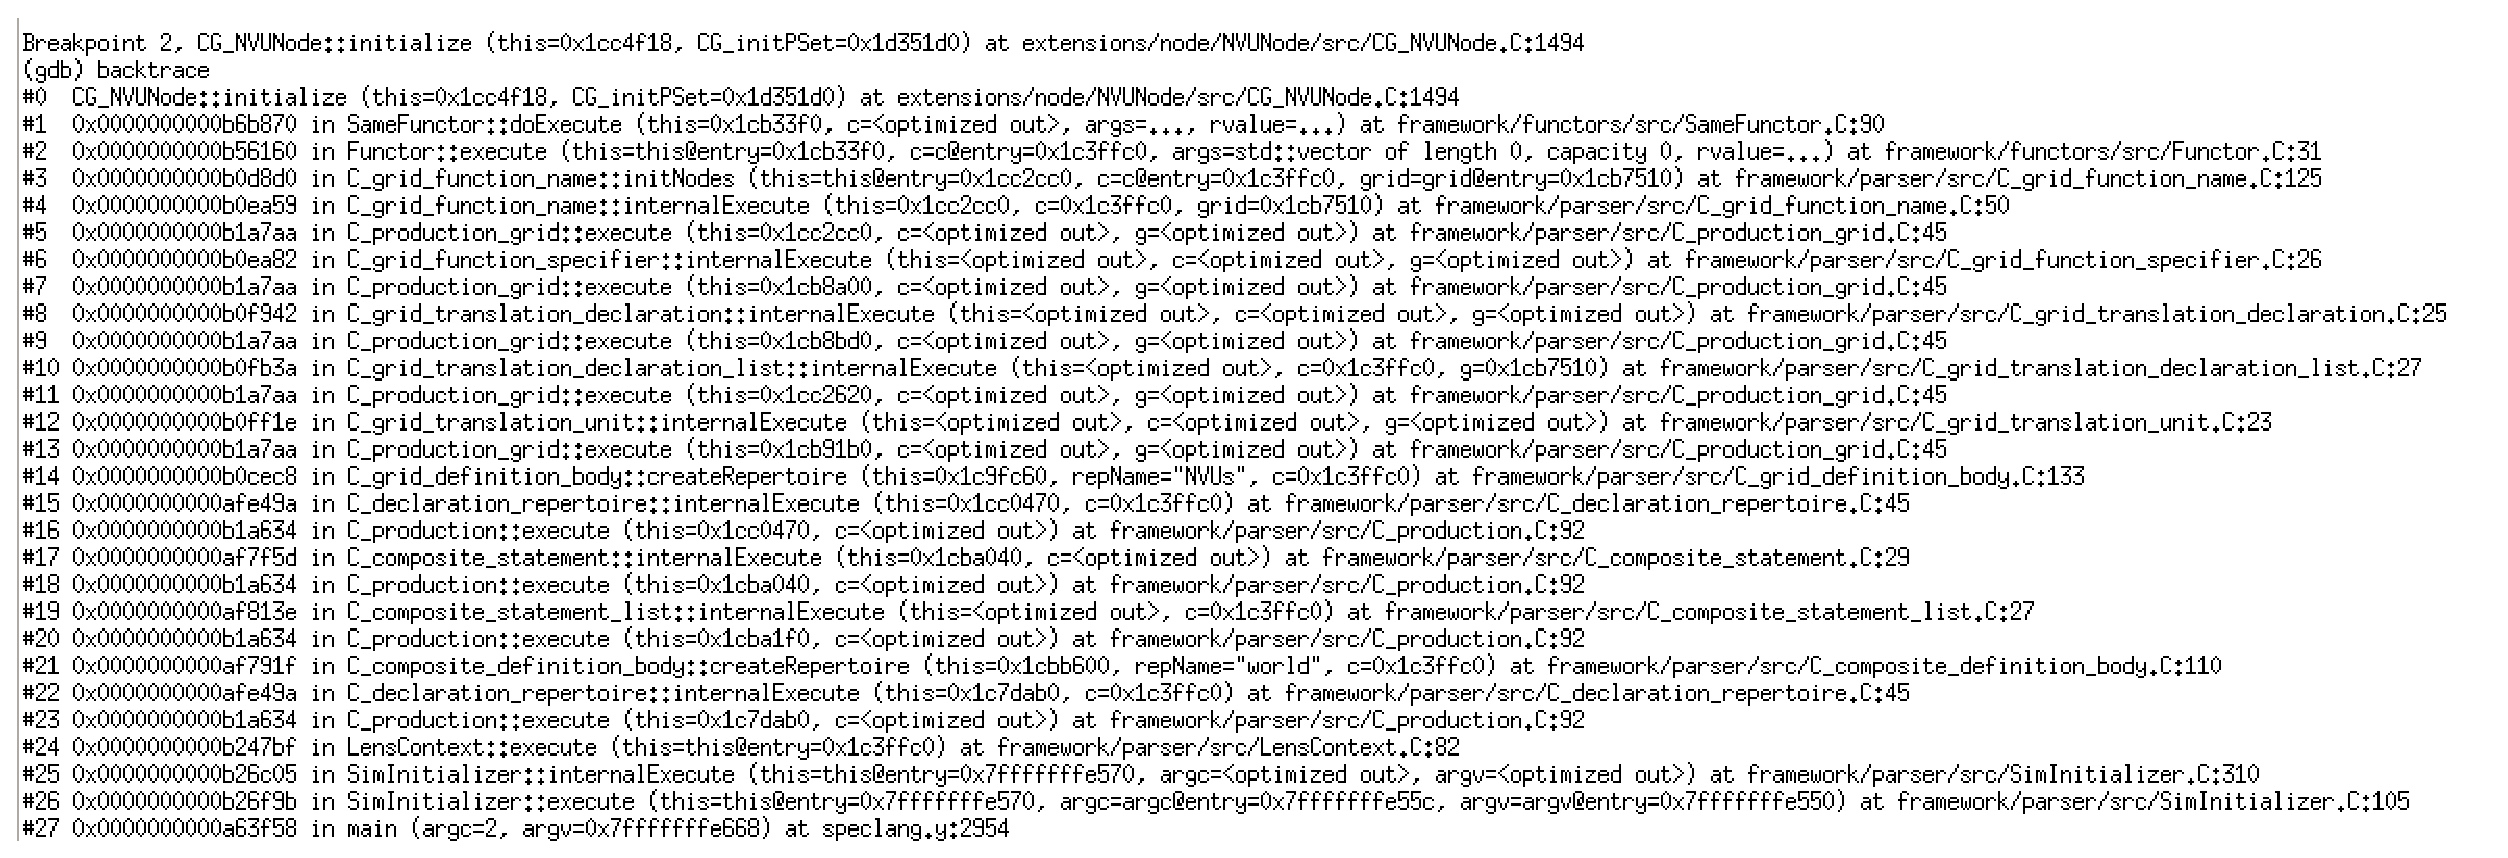
\includegraphics[height=5cm,
    angle=0]{./images/MGS_execution_order.eps}}
\caption{Execution order in MGS framework which call
CG\_NVUNode::initialize() before calling the NVUNode::initialize()}
\label{fig:MGS_execution_order}
\end{figure}


At the end of each phase, during the real simulation, the graph-based framework
will make some data exchange before reaching to the next phase.


\subsection{EdgeConnection}
\label{sec:MDL-EdgeConnection}

This concept is used when EDGE is treated as an entity like NODE, CONSTANT
\ldots. However, this is no longer needed.

This concept is obsolete and should be removed from the grammar
\begin{verbatim}
// this is not being used
   76 edgeConnection: CONNECTION PRE NODE '(' ')' EXPECTS interfacePointerList '{' edgeConnectionStatementList '}'
   77               | CONNECTION POST NODE '(' ')' EXPECTS interfacePointerList '{' edgeConnectionStatementList '}'
   78               | CONNECTION PRE edgeConnectionComponentType '(' ')' EXPECTS interfacePointerList '{' connectionStatementList '}'
   79               | CONNECTION PRE edgeConnectionComponentType '(' predicate ')' EXPECTS interfacePointerList '{' connectionStatementList '}'

\end{verbatim}
Check the \verb!mdl.output! file.

\subsection{Connection}
\label{sec:MDL-Connection}

The kinds of connection a component (NODE, CONSTANT, VARIABLE) expects should be
defined as definition time. 

\begin{verbatim}
   86 connection: CONNECTION PRE connectionComponentType '(' ')' EXPECTS interfacePointerList '{' connectionStatementList '}'
   87           | CONNECTION PRE connectionComponentType '(' predicate ')' EXPECTS interfacePointerList '{' connectionStatementList '}'

   88 connectionComponentType: NODE
   89                        | EDGE
   90                        | CONSTANT
   91                        | VARIABLE
\end{verbatim}
NOTE: \verb!EDGE! is obsolete concept.

We can create a directed connection between a (post) NODE  
\begin{enumerate}
  \item to a (pre) NODE
  \item to a (pre) CONSTANT 
  \item to a (pre) VARIABLE
  \item to a (pre) EDGE  [should not be used]
\end{enumerate}


A connection between two nodes is defined in the form of
\begin{verbatim}

Connection Pre Node () Expects AmplitudeProducer {
   // ...
}


Connection Pre Node (predicate_as_some_boolean_test) Expects AmplitudeProducer {
   // ...
}

\end{verbatim}

\begin{enumerate}
  \item The direction of the connection: \verb!Pre Node! or \verb!Post Node!
  
 IMPORTANT: Currently, \verb!Post Node! is disabled, i.e. not necessary as the
 connection is directed (i.e. if A is pre of B then implicitly B is post of A).
 
  \item \verb!Some_boolean_test! (optional): a condition (i.e. predicate)
  telling when the connection is established (Sect.\ref{sec:MDL-predicate})


  \item When a node connects to a pre-node, it expects to receive something
  from that pre-node which is defined through a common Interface, e.g. 
  \verb!AmplitudeProducer! interface in the below example
  
\begin{verbatim}

Connection Pre Node (PSet.identifier == "FF") Expects AmplitudeProducer {
   AmplitudeProducer.somevalue >> mydata;  // write to the right side
}
\end{verbatim}

It means the pre-Node doesn't care which (post)node connects to it. 
Depending on the design of the interface (it's data member is a pointer or not),
the (post)node can have direct access to the data member in the pre-node, giving
that the two node instances are on the same memory space (as if they are on the
different memory space)

The (post)node can have read-access, and 
However, it's
important that the (post)Node should not expect to modify any data

  \item 
  
  \item In the body of the Connection, we define the mapping between the output
of the Pre (Node/Value/Constant) and the current data member.

NOTE: In the generated code, these definitions are stored in InterfaceToMember
and PSetToMember classes.


\end{enumerate}

{\bf Example:} Consider the scenario
 \begin{verbatim}
 Node_LifeNode_instance_1 ----------> Node_LifeNode_instance_2
 \end{verbatim}
 Then, the statement below means that \verb!Node_LifeNode_instance_2! will
 receive the input from \verb!Node_LifeNode_instance_1! and put that to the data
 member \verb!neighbors!.

\begin{verbatim}
Node LifeNode Implements ValueProducer {
   int value;
   int publicValue;
   int* [] neighbors;

   Connection Pre Node () Expects ValueProducer {
      ValueProducer.value >> neighbors;
   }
}
\end{verbatim}

\textcolor{red}{\bf TIPS}: The data member storing the input values from
incoming Nodes is defined as an array. Here, we use an array pointer meaning
that we don't do deep copy, but we do referencing to the data, i.e. shallow
copy, which is a good way to reduce the cost of copying data.

NOTE: In the above example, a Node component both input and output the same type
of information. If it input information A, but output information B, typically
that node does not connect to a node of the same type
\begin{verbatim}
Node TypeA Implements Value_1_Producer {
  int* [] internal_data;

 Connection Pre Node () Expects Value_2_Producer {
     Value_2_Producer.somedata >> internal_data;
 }

}

Node TypeB Implements Value_2_Producer {

}
\end{verbatim}

Keywords:
\begin{verbatim}
Connection
Pre { Node/Variable/Constant}
Post { Node/Variable/Constant}
Expects
\end{verbatim}

  As a Node ``A" doesn't know what data the connected Node ``B" provides, it
  needs to rely on the Interface of Node ``B'' 

  
\subsection{Functor}
\label{sec:Functor-in-MDL}


MDL can help us to generate a code stub for a functor creator
(Sect.\ref{sec:Functor-MGS}, what we need to provide is telling the
\verb!<Functor-name>!, the proper category, along with the interface for the two
methods \verb!Initialize! and \verb!Execute!
\begin{itemize}
  \item we don't care about the return value of Initialize as it is being used
  in the constructor for the functor
   
  \item we can have different inputs and return type for the Execute()
\end{itemize}

EXPLAIN:
\begin{verbatim}
// Option 1:
Framework  Functor <Functor-Name>  {

} 

// Option 2:
Framework  Functor <Functor-Name>  Category "<choose-one>" 
{
  /* define what function you want to implement 
     using the names 
      'Initialize'  --> map to doInitialize(...) in C++ generated code 
      'Execute'     --> map to doExecute(...) in C++ generated code
     and you are free to choose how the input should be 
     and how the returned value should be 
     (as you are the one to use it)
  */
  
}
\end{verbatim}


Example: TissueConnectorFunctor.mdl
\begin{verbatim}
#ifndef TissueConnectorFunctor_MDL
#define TissueConnectorFunctor_MDL

Framework Functor TissueConnectorFunctor Category "CONNECTOR" {
   Initialize();
   void Execute();
}

#endif
\end{verbatim}

Example: TissueFunctor.mdl (Sect.\ref{sec:TissueFunctor.mdl})
\begin{verbatim}
#ifndef TissueFunctor_MDL                                                                                                                                                                           
#define TissueFunctor_MDL                                                                                     
                                                                                                              
Framework Functor TissueFunctor Category "FUNCTOR" {                                                          
   Initialize(string commandLineArgs1, string commandLineArgs2, string compartmentParamFile, 
             string channelParamFile, string synapseParamFile, 
             Functor* layoutFunctor, Functor* nodeInitFunctor, 
             Functor* connectorFunctor, Functor* probeFunctor);
   Functor* Execute(string tissueElement, NDPairList* params);                                                
}                                                                                                             
                                                                                                              
#endif                                                                                                        
\end{verbatim}

Example: TissueProbeFunctor.mdl
\begin{verbatim}
#ifndef TissueProbeFunctor_MDL                                                                                                                                                                      
#define TissueProbeFunctor_MDL                                                                                
                                                                                                              
Framework Functor TissueProbeFunctor {                                                                        
   Initialize();                                                                                              
   NodeSet* Execute();                                                                                        
}                                                                                                             
                                                                                                              
#endif
\end{verbatim}

Example:
\begin{verbatim}
Framework Functor TissueProbeFunctor {
   Initialize();
   NodeSet* Execute();
}
\end{verbatim}

Example: TissueFunctor (Sect.\ref{sec:TissueFunctor})
{\tiny
\begin{verbatim}
Framework Functor TissueFunctor Category "FUNCTOR" {
   Initialize(string commandLineArgs1, string commandLineArgs2, string compartmentParamFile, 
             string channelParamFile, string synapseParamFile, 
             Functor* layoutFunctor, Functor* nodeInitFunctor, 
             Functor* connectorFunctor, Functor* probeFunctor); 
       
   Functor* Execute(string tissueElement, NDPairList* params);
}
\end{verbatim}
}

Now, we use \verb!mdlparser! to generate the C++ code stub which is stored in a
folder with the same name of the given functor-creator-name, under the location
given in Sect.\ref{sec:functor-location-of-user-defined-functor-creator-in-GSL}.

% Some built-in functors already have C++ code implemented in
% GSL/framework/functor (Sect.\ref{sec:functors-in-MGS-framework}).



\begin{enumerate}
  \item pre-processor by the preprocessor \verb!cpp! to create a completed MDL file.
  
Those passed via the \verb!-i! argument, with colon (:) separated list, are the folders where it searches for header files  
  
  \item \verb!<MdlLexer>! scanner - Sect.\ref{sec:MdlLexer-class}
  
the scanner scan the completed MDL files, and generate the tokens to be used by the MdlContext object.

For parsing, the content of this final MDL file is stored in a temporary file.
The name and location of temporary file depends upon the system BLUE-GENE or AIX
or LINUX. 

\textcolor{red}{NOTE: A similar process can be referenced in Sect.\ref{sec:parse-gsl-file}}.

  \item \verb!<MdlContext>! context
  
\begin{verbatim}
// class MdlContext {
//   MdlLexer * _lexer;
//   MemberContainer<Generatable> *_generatables;
// }

context->_lexer = scanner.get();

// which holds the vector of 'Generatable' type
_generatables = new MemberContainer<Generatable>();

context->_genetables = _generatables;

\end{verbatim}  
Generatable class - Sect.\ref{sec:Generatable-class}

\section{Generating C++ code}

Once the grammar is read-in and the contextual information are stored in proper
class's objects, now is the step to generate C++ code.

\subsection{MemberContainer}
\label{sec:MemberContainer}

NOTE: \verb!MemberContainer! is a dictionary-like container
(Sect.\ref{sec:MemberContainer}) with key is the name as defined in MDL (e.g.
LifeNode), and value is a \verb!Generatable! object which holds all information
we need to generate C++ code for that key-name.
\begin{verbatim}
// in MDL file
Node LifeNode Implements ValueProducer {
   // ...
}
\end{verbatim}
then key would be '\verb!LifeNode!' string.

   \item \verb!mdlparse(void*)!  is the function that parse the MdlContext object
   
   
\begin{verbatim}
extern int mdlparse(void*);


mdlparse(context.get());
\end{verbatim}
\end{enumerate}


\subsection{* Step 1}
\label{sec:MDL-how-it-works-step-1}

A script \verb!*.mdl! file may contains one or more components
(Sect.\ref{sec:MDL-component}).


Based on the type of different components defined by user in *.mdl file, the
tool generate an appropriate C++ code which are put into different subfolders (e.g.
LifeNode/, LifeDataCollector/, ValueProducer/ in the Game of Life project) of 
\verb!./gsl/extensions/<component-type>/!.
The content of these folders (including files and folder creation) are taken
care by the below classes.

\verb!./mdl/include/Class.h! contains the class \verb!Class! that encapsulate
C++ code definition and generation for a given *.mdl file. The information from
an instance of this class is used to generate 2 files:
header file and source file. It generates,
\begin{itemize}
  \item header file: the class definition for the model
  
  
  \item source file: the implementation for the model, which includes
  \begin{enumerate}
    \item user-defined methods and attributes
    
 \textcolor{red}{NOTE}: user needs to modify and implement these methods
 approriately. 
 
 Methods are classified into two types:
 \begin{itemize}
   \item methods with predicate that serve as kernel accepting input from
   another component (Node/Variable/Constant)
   
   \item methods without predicate: the execution of these methods
   are independent from other components (Node/Variable/Constant), however,
   there can be order between them in the same component.
   
   
   These methods are classified into 3 types
   \begin{enumerate}
     \item user function:
     define work to be done when a connection is accepted.
     
     Am empty function will be generated and the user is going to fill
     in using C++ to implement the behavior of the component. 
     
     \item triggered function
     
     \verb!TriggeredFunction! methods:
%       (\textcolor{red}{obsolete}, triggers are built in,
%      under framework/dca):
     these methods do not run every iteration, rather they are only run if a
     trigger fires, i.e. a condition is satisfied.
     
     Triggered functions can be defined serial or parallel, serial ones are run
     at the beginning of the phase, single threaded.  Parallel triggered
     functions are run with the rest of the work in the phase.
     
     
     \item phase function: these functions run depending on which phase of the
     simulation (Sect.\ref{sec:GSL-phase-simulation})
     
   \begin{enumerate}
     \item \verb!InitPhase! methods:
     these methods run only one time, right after the parser is done
     
     \item \verb!RuntimePhase! methods: 
     these methods run every time-step
    
     NOTE: The time-step is pre-configured and is fixed.
     
     \item \verb!LoadPhases! methods:
     these methods are executed after the simulation does a restore operation.
     
     \item \verb!FinalPhase! methods:
     these methods run once, after the simulation is completed and before memory
     is freed.
     

   \end{enumerate}
 \end{enumerate}
   NOTE: Subscriber (Obsolete)
   
 \end{itemize}

 
    \item basic methods: e.g. constructor, duplicate method, copy constructor,
    destructor \ldots
  \end{enumerate}

For macro definition in these two files, 
\verb!./mdl/include/MacroConditional.h! contains the class
\verb!MacroConditional! that encapsulate how 
\verb!#ifdef ... #endif! statements are inserted into these files.
An instance of this class, with an appripriate input argument, can generate the
proper \verb!#ifdef ... #endif! statement.

\end{itemize}


The information about the definition of Connection between two components
(Node/Variable/Constant) are stored in InterfaceToMember and
PSetToMember classes.
\begin{verbatim}
./mdl/include/PSetToMember.h
./mdl/include/InterfaceToMember.h
\end{verbatim}

 
 \subsection{-- code help generate methods}
 
 Code for helping generating the methods are defined in
 \verb!./mdl/src/Method.C!.
 \begin{verbatim}
 mdl/src/ConstructorMethod.C  
 mdl/src/CopyConstructorMethod.C 
 mdl/src/DefaultConstructorMethod.C  
 mdl/src/Method.C
 \end{verbatim}
 DefaultConstructorMethod and CopyConstructorMethod inherit from
 Constructor Method.
 
 
 \subsection{-- code help generate attributes}
 
 Code for helping to generate attributes are defined in
 \begin{verbatim}
 mdl/src/Attribute.C  
 mdl/src/CustomAttribute.C  
 mdl/src/DataTypeAttribute.C
 \end{verbatim}
 
 \subsection{-- code help mapping MDL type to C++ type}
 
 Code for mapping MDL data type to C++ data type is defined in
 \begin{verbatim}
 mdl/src/DataType.C
 mdl/src/DataTypeAttribute.C  
 \end{verbatim}
 
 \subsection{-- code help generate predicate}
 
 Code for predicate
 \begin{verbatim}
 mdl/src/Predicate.C 
 mdl/src/FunctionPredicate.C  
 mdl/src/InstancePredicate.C  
 mdl/src/PredicateException.C  
 mdl/src/PredicateFunction.C  
 mdl/src/PSetPredicate.C  
 mdl/src/SharedPredicate.C
 \end{verbatim}
 
 specify modification of model values or shared variable values according to run
 time predicates
 \begin{verbatim}
 Predicate class
   |
   PSetPredicate
   
 \end{verbatim}
 
 \subsection{-- code for operation}
 
\begin{verbatim}
mdl/src/Operation.C
mdl/src/InFixOp.C
mdl/src/TerminalOp.C
mdl/src/ParanthesisOp.C
\end{verbatim}


\subsection{* Step 2}

A script file and a .mk file are also generated
\begin{verbatim}
copyModules
Extensions.mk
\end{verbatim}

The content of the above files are generated based on the
\verb!Initializer! class defined in
\begin{verbatim}
../../mdl/include/Generatable.h:      // Fills in the map with itself; used for copyModules.
../../mdl/include/Initializer.h:      std::map<std::string, std::vector<std::string> > _copyModules;
../../mdl/src/Initializer.C
\end{verbatim}

\subsection{* Step 3}

The script \verb!./models/define! is run which execute the script
\verb!copyModules! to copy the generated C++ code to different folders inside
\verb!./gsl/extensions/!



\subsection{* Step 4}

The C++ generated code, as mentioned in Step 1, are
\begin{itemize}
  \item \verb!CG_*.c! files: about 99\% (CG = code-generated)
  
  \item \verb!*.c.gen! files: about 1\%. These are also code-generated file, but
  the content need to be modified and updated by user (i.e. implement the
  behavior you need).
  
  You need to remove the \verb!.gen! extension in \verb!.h.gen.! and 
  \verb!.C.gen! files and write codes.
  
\end{itemize}

These code will be used by GSL (Sect.\ref{sec:GSL}), if the component is being
used in the \verb!*.gsl! script.


\subsection{Generatable}
\label{sec:Generatable-class}

A \verb!Generatable! represents a component, with all necessary information,
that can be used to generate into a C++ source file (i.e. \verb!CG_*! files and
\verb!*.h.gen!, \verb!*.C.gen! file).

\verb!Generatable! is an abstract class, and depending on the type of component
we want to generate, the run-time object can be an instance of 
\begin{enumerate}
  \item \verb!Node! class
  
  \item \verb!Interface! class
  
  \item \verb!InterfaceImplementorBase! class
  
  From which many further class is derived
\begin{verbatim}
Node <--  SharedCCBase  <--   ConnectionCCBase  <--   CompCategoryBase  <-- InterfaceImplementorBase
\end{verbatim}
  
  \item \verb!StructType! class 
  
  \item \verb!ToolBase! class 
\end{enumerate}

\subsection{-- Node: SharedCCBase : ConnectionCCBase : CompCategoryBase : InterfaceImplementorBase : Generatable}
%\label{sec:Node-MDL}

A \verb!Node! is a generatable (Sect.\ref{sec:Node-MDL}). This class is used for
generating different C++ code from MDL definition of a construct (e.g. node,
edge, interface, struct, \ldots).

\begin{mdframed}

Suppose you define this in MDL
\begin{verbatim}
// in MDL file
Node LifeNode Implements ValueProducer {
   // ...
   int value;
}
\end{verbatim}

then a \verb!Node! object (a generatable object) is created, along with that is all functions will be evoked to create supporting classes (CG\_*) for this node 
(Sect.\ref{sec:MDL-generated-classes}).

It will be generated into  a folder structure to put it into \verb!./gsl/extensions/<one-of-10-family>/!, e.g.
\begin{verbatim}
./gsl/extensions/node/LifeNode/include/LifeNode.h.gen
                                       CG_....h
                              /src/LifeNode.C.gen
                                   CG_.....C
                              /obj/
                              /module.mk
\end{verbatim}

To do that, e.g. for the construct of node type,
there is a class, e.g. a Node class derived from \verb!Generatable!
(direct or indirect), (2) and implement the \verb!internalGenerateFiles()!
method.
\end{mdframed}

The two importants methods are
\begin{enumerate}
  
  \item  \verb!generate()! (virtual function) called first to prepare the
  internal content, and output the (not-so-exact) MDL code into standard output
  
  Some data for array is transformed into \verb!ShallowArray! such as what given
  in Sect.\ref{sec:Node-MDL-2-C++-code-generated}.
  
  \item \verb!generateFiles()!:  create all \verb!CG_*! files (must be called after \verb!generate()! is completed)
  \label{sec:Generatable-generateFiles}
  
It's important to check internalGenerateFiles() from Node (Sect.\ref{sec:Node-MDL-2-C++-code-generated}),
from Interface (Sect.\ref{sec:Interface-MDL}).

\begin{verbatim}
Generatable::generateFiles(... /* MDL file_name */)
{
  internalGenerateFiles(); //to be implemented by different subclass of Generatable

  createDirectoryStructure();  // create folders
         // e.g. ValueProducer/
         //      ValueProducer/src
         //      ValueProducer/include
         //      ValueProducer/obj
         //      

 for (std::vector<Class*> ...
    )
 {
   //type(*it) == Class class [so check this class]
   (*it)->setFileOutput(_fileOutput); // true or false flag
   (*it)->generate(getModuleName()); // this is the one that really generate C++ code (to multiple files if _fileOutpue=True)
 }

}
\end{verbatim}
Class class - Sect.\ref{sec:Class-mdl} has \verb!generate()! method.


\end{enumerate}
Other methods are defined in the derived classes (see below for the class names).

%generation purpose (e.g. Sect.\ref{sec:MdlLexer-class} - Sect.\ref{sec:Initializer-execute()}). 



Derived class: \textcolor{red}{IMPORTANT: Those with asterisk (*) are those that implements methods to generate C++ code from 
the corresponding MDL construct}
\begin{verbatim}
Generatable
  |
  ToolBase
     |
     Functor*
         |
         CG_TissueFunctorBase
            |
            TissueFunctor    

Generatable
  |
  Interface*
      |
      CompCategoryBase

Generatable, DataType
  |
  StructType*
    
Generatable
  |
  InterfaceImplementorBase
     |
     CompCategoryBase
     |   |
     |   ConnectionCCBase
     |      |
     |      SharedCCBase
     |      |   |
     |      |   Edge*
     |      |   |
     |      |   Node*
     |      |
     |      Variable*
     Constant*
\end{verbatim}

EXPLAIN:
\begin{enumerate}
  \item Node (Sect.\ref{sec:Node-MDL-2-C++-code-generated}) handles the creation of C++ code for the MDL component defined as \verb!Node!
  
\begin{verbatim}
Node LifeNode Implements ValueProducer {
}
\end{verbatim}
  
  \item Interface (Sect.\ref{sec:Interface-MDL})  handles the creation of C++ code for MDL component defined as \verb!Interface!
  
  
  
  \item SharedCCBase (Sect.\ref{sec:SharedCCBase}), 

  \item InterfaceImplementorBase -
  Sect.\ref{sec:InterfaceImplementorBase::getAddConnectionFunctionBody()}
  handles the creation of C++ code for the interfaces (that comes after
  \verb!Implements! keyword), e.g. \verb!ValueProducer!.
  
  \item \verb!CompCategoryBase! handles the creation of C++ code representing \verb!LifeNode!CompCategory class(es)

\begin{verbatim}
class CG_LifeNodeCompCategory

class LifeNofdeCompCategory
\end{verbatim}
  
  \item \verb!ConnectionCCBase! handles the creation of C++ code to support connection (receiving input, exposuring data)
\end{enumerate}

\textcolor{red}{C++ code}: 
\begin{verbatim}
class Generatable
{
public:
      enum LinkType {_DYNAMIC, _STATIC};  //whether the CG_* will be linked
                     //static or dynamic

protected:
	virtual void internalGenerateFiles() = 0;
	
	virtual void generate() const = 0;
	
	void generateModuleMk(); // generate module.mk file
	   // this method is supposed to be read-in by the Makefile
	   // so that it generate static-link (e.g. ValueProducer.a)
	   // or a shared-library (e.g. ValueProducer.so)
	   //  at MDL single construct level
	   //  this would generate so many libraries, unfortunately for this approach
	   // NOTE: It is not being used right-now


      // The classes that this generatable has.
      std::vector<Class*> _classes;
      // Write to disk if true.
      bool _fileOutput;

private:
      // The filename the generatable was read from. More specifically
      // the components(generatables) in .mdl files which are 
      // #included do not generate the actual files.
      std::string _fileName; 
      LinkType _linkType;
}
\end{verbatim}

\subsection{DataItem: ConstantDataItem}
\label{sec:DataItem}

Any data defined in MDL are treated as a vector of one (in the case of scalar)
or many (in the case of array) to \verb!DataItem! (Sect.\ref{sec:gsl-dataitems})
in the GSL framework.

A DataItem is just a way to wrap the 'real type' of the data. Example:
\begin{verbatim}
class RepertoireDataItem : public DataItem
{
  protected:
  Repertoire * _repertoire;
  
  public:
  Repertoire* getRepertoire() const;
  void setRepertoire(Repertoire *);  
}
\end{verbatim}

DataItem provides 2 universal methods that can be used to query the exact
data type it holds
\begin{verbatim}
class DataItem
{

  public:
  virtual const char* getType() const;
  virtual std::string getString(Error* error=0) const;
}
\end{verbatim}

\subsection{-- ConstantDataItem}
\label{sec:ConstantDataItem}


\begin{lstlisting}
class Constant;

class ConstantDataItem : public DataItem
{

   private:
      Constant *_data;
  public:
      static char const* _type;

     const char* getType() const;

}
\end{lstlisting}

\subsection{*** Constant}
\label{sec:Constant-MDL-C++}

\begin{lstlisting}
class Constant : public InterfaceImplementatorBase
{

}
\end{lstlisting}

\subsection{StructDataItem}
\label{sec:StructDataItem}

\begin{lstlisting}
class Struct;

class StructDataItem : public DataItem
{

   private:
      Struct *_data;
...
}
\end{lstlisting}

\subsection{*** Struct}
\label{sec:Struct-MDL-C++}

It's a virtual class, with no specific data, and that enable user to put any
thing here. Data is always organized as a vector of DataItem
(Sect.\ref{sec:DataItem})
\begin{lstlisting}
class Struct
{

}
\end{lstlisting}
\subsection{Class factories: InstanceFactory}
\label{sec:InstanceFactory}

\begin{verbatim}
class InstanceFactory
{

  protected:
      std::vector<std::vector<std::pair<std::string, DataItem*> > > _parameterDescription;
      std::vector<DataItem*> _instances;
   private:
      void copyOwnedHeap(const InstanceFactory& rv);
      void destructOwnedHeap();

}
\end{verbatim}

Simulation object (Sect.\ref{sec:Simulation-class-GSL}), has a vector of 
\begin{verbatim}
std::vector<InstanceFactoryRegistry*>  _instanceFactoryRegistries;
\end{verbatim}


\subsection{-- StructureType}
\label{sec:StructureType}


\subsection{-- ConstantType}
\label{sec:ConstantType}

We use the class factories (Sect.\ref{sec:InstanceFactory}) mechanism to either
(1) create an instance for the associated MDL component, e.g.
Sect.\ref{sec:ConstantType-create-instance}

\begin{verbatim}
class ConstantType : public InstanceFactory
{
protected:
    DuplicatePointerArray<Constant> _constantList;

public:
 virtual void getConstant(std::auto_ptr<Constant> & r_aptr)=0;
      virtual Constant* getConstant()=0;
      virtual std::string getName()=0;
      virtual std::string getDescription()=0;
      
      virtual void getInstance(std::auto_ptr<DataItem> & adi, 
			       std::vector<DataItem*> const * args, 
			       LensContext* c);
      virtual void getInstance(std::auto_ptr<DataItem> & adi, 
			       const NDPairList& ndplist,
			       LensContext* c);      
}
\end{verbatim}


\subsection{-- RepertoireDataitem}
\label{sec:RepertoireDataitem}

A DataItem is just a way to wrap the 'real type' of the data. Example:
\begin{verbatim}
class RepertoireDataItem : public DataItem
{
  protected:
  Repertoire * _repertoire;
  
  public:
  Repertoire* getRepertoire() const;  
}
\end{verbatim}

\section{C++ generated code for MDL script}
\label{sec:MDL-generated-classes}

Consider the \verb!HodgkinHuxleyVoltage! Node defined in *.mdl
(Sect.\ref{sec:HodgkinHuxleyVoltage-mdl-code}), there will be a number of
generated classes, among them are two user-modifiable classes
\begin{itemize}
  \item HodgkinHuxleyVoltage (Sect.\ref{sec:HodgkinHuxleyVoltage-C++-code})
  \item HodgkinHuxleyVoltageCompCategory
  (Sect.\ref{sec:HodgkinHuxleyVoltageCompCategory})
\end{itemize}

\begin{lstlisting}
class HodgkinHuxleyVoltage { } // user can modify

class CG_HodgkinHuxleyVoltage  // the proxy for connecting the real
                               // implementation in HodgkinHuxleyVoltage
                               // to the GSL Framework 

class CG.................... Pset
............................ Proxy
............................ Factory
............................ Publisher
............................ InAttrPset
............................ OutAttrPset
............................ CompCategory
............................ NodeAccessor
............................ GridLayerData
............................ SharedMembers
............................ WorkUnitShared
............................ WorkUnitInstance
............................ ProxyDemarshaller
............................ TriggerableCaller
............................ WorkUnitGridLayers

class HodgkinHuxleyVoltageCompCategory
\end{lstlisting}

Explains:
\begin{enumerate}
  \item InAttrPset: the class contains data members defined in the
  \verb!InAttrPset! section
  
  \item OutAttrPset: \ldots (just not being used) \verb!OutAttrPset! section
  
  \item SharedMembers: \ldots \verb!Shared! section
  
  \item CompCategory: Whenever that given component (e.g. NodeType) is being
  used in the GSL, then the GSL framework will call this class of that component
  to create an array of instances of that component. So this class is a
  container for the instance of the corresponding 
\end{enumerate}

A generatable of class \verb!Node! - Sect.\ref{sec:Node} (Sect.\ref{sec:Generatable-class}) 


\subsection{CG\_...CompCategory class}

This class is important for each generated NodeType, as it 
is the factory class, that hold 
\begin{enumerate}
  \item  how many instances of that NodeType to create (on a local computing
  node)

  \item how to initialize Shared data for all instances of that NodeType (on a
  local computing node).
  
  \item how to perform Marshaller and Demarshaller when data are stored across
  the memory spaces on different computing nodes is requested.
\end{enumerate}

\subsection{-- LifeNodeCompCategory}


Suppose MDL
\begin{verbatim}
Node LifeNode 
{
   int value;      //anything here becomes part of LifeNode class
   int[] somedata;
   
   Shared {  
      int tooParse; // any data member inside Shared
                 // are part of CG_...ShareMembers.h 
      InitPhase initSharedData; // anything method inside Shared 
                       // become parts of CG_LifeNodeCompCategory class 
   }
   
   InitPhase initData();
}
\end{verbatim}

\begin{lstlisting}
class LifeNodeCompCategory: public CG_LifeNodeCompcategory
{
public:
 LifeNodeCompCategory(Simulation& sim, 
             const std::string& modelName, 
             const NDPairList& ndpList);

}

class CG_LifeNodeCompCategory 
{
public:
   int tooParse;
   ShalllowArray<LifeNode, 1000, 4> _nodes; // linked-list to all instances
               // of the NodeType LifeNode to be created for a given
               // model simulation
   ConnectionIncrement _computeCost;
   
}

\end{lstlisting}


\subsection{-- HodgkinHuxleyVoltageCompCategory}
\label{sec:HodgkinHuxleyVoltageCompCategory}


{\small
\begin{lstlisting}
class HodgkinHuxleyVoltageCompCategory : public
                CG_HodgkinHuxleyVoltageCompCategory, public CountableModel {
   public:
      HodgkinHuxleyVoltageCompCategory(Simulation& sim, const std::string& modelName, const NDPairList& ndpList);
      void count();
};


class CG_HodgkinHuxleyVoltageCompCategory {
 
protected:
#ifdef HAVE_MPI
      std::map <int, CCDemarshaller*> _demarshallerMap;
#endif
#ifdef HAVE_MPI
      std::map <int, CCDemarshaller*>::iterator _demarshallerMapIter;
#endif
#ifdef HAVE_MPI
      std::map <int, ShallowArray<CG_HodgkinHuxleyVoltage*> > _sendMap;
#endif
#ifdef HAVE_MPI
      std::map <int, ShallowArray<CG_HodgkinHuxleyVoltage*> >::iterator _sendMapIter;
#endif


    ShallowArray<HodgkinHuxleyVoltage, 1000, 4> _nodes;
    ConnectionIncrement _computeCost;
 
}

\end{lstlisting}
}

Here, we need to implement \verb!::count()! method
(Sect.\ref{sec:CountableModel}) which basically returns the total number of
instances created/allocated across all MPI ranks. NOTE: An instance represent
one representation for that component, e.g. ChannelNat, for one compute-branch
(Sect.\ref{sec:ComputeBranch}).
This needs to be implemented at xxxCompCategory class level, as this is where it
keeps track of all instances to be allocated for one MPI process.


\subsection{Implement C++ code HodgkinHuxleyVoltage}
\label{sec:HodgkinHuxleyVoltage-C++-code}

TIPS:
\begin{enumerate}
  \item to get access to shared data among instances of one Node type
  
\begin{verbatim}
 // MDL: Shared{ float * deltaT;}
 // to get to the value in C++
*(getSharedMembers().deltaT)

 // MDL: Shared {float Ra;}
getSharedMembers().Ra
\end{verbatim}  
  
  
\subsection{Implement C++ code: NaChannel}
\end{enumerate}


\subsection{UserFunction}
\label{sec:UserFunction}


A UserFunction, e.g. 
{\tiny
\begin{lstlisting}
  InAttrPSet {  // the attribute of the incoming MDL's component
                // which will be used to check for connection 
    string identifier;
    TissueSite site;
    int idx;
  }

UserFunction setReceptors, setInjectedCurrent;

  // i.e. oh, the 'Node' connecting to the current node
  //   must have the attribute 'identifier' whose value is
  //                    'electricalSynapse[Voltage]
  // NOTE: TissueFunctor will assign the value to 'identifier' to the right
  //         component using
  /*
   std::map<std::string, NDPairList> esyn2cpt;
 
    os.str("");
    NDPairList Mesyn2cpt;
    os << "electricalSynapse[" << cptVarTypesIter->first << "]";
    Mesyn2cpt.push_back(new NDPair("identifier", os.str()));
    Mesyn2cpt.push_back(new NDPair("idx", 0));
    esyn2cpt[cptVarTypesIter->first] = Mesyn2cpt;
  
  */
 Connection Pre Node (PSet.identifier=="electricalSynapse[Voltage]") Expects CurrentProducer {
    CurrentProducer.current >> injectedCurrents.current;
    setInjectedCurrent();
   }

  Connection Pre Node (PSet.identifier=="chemicalSynapse[Voltage]") Expects ConductanceProducer, ReversalPotentialProducer {
    ConductanceProducer.conductance >> receptorCurrents.conductance;
    ReversalPotentialProducer.reversalPotential >> receptorCurrents.reversalPotential;
    setReceptorCurrent();
   }
\end{lstlisting}
}
is converted to C++ method which has all the arguments we need to get access to
the graph-based framework
\begin{lstlisting}
void CG_HodgkinHuxleyVoltage::setInjectedCurrent(
        // can be: "Pre", "Post"
        const String& CG_direction,
        // can be: "Variable", "Node", ... 
        const String& CG_component,
        // depending on the value of CG_component, one should be set
        // and the other will be 0
        NodeDescriptor* CG_node, 
        Edge* CG_edge, 
        VariableDescriptor* CG_variable, 
        Constant* CG_constant,
        // InAttrPSet of the incoming
        //    to use: CG_inAttrPset->identifier
        // if MDL has InAttrPSet{ string identifier;} for example
        CG_HodgkinHuxleyVoltageInAttrPSet* CG_inAttrPset,
        // OutAttrPSet of the outgoing
        CG_HodgkinHuxleyVoltageOutAttrPSet* CG_outAttrPset
        ) {};

void HodgkinHuxleyVoltage::setReceptorCurrent(const String& CG_direction, 
        const String& CG_component, NodeDescriptor* CG_node, 
        Edge* CG_edge, VariableDescriptor* CG_variable, Constant* CG_constant,
        CG_HodgkinHuxleyVoltageInAttrPSet* CG_inAttrPset,
        CG_HodgkinHuxleyVoltageOutAttrPSet* CG_outAttrPset
        ) 
{
}

\end{lstlisting}

Example: when it is called in the C++ generated code
\begin{verbatim}
 setInjectedCurrent("Pre", "Variable", 0, 0, CG_variable , 0, CG_castedPSet, 0);
\end{verbatim}
and then needs to be implemented in the derived class


\subsection{PredicateFunction}
\label{sec:PredicateFunction}

\begin{verbatim}
Node HodgkinHuxleyVoltage{
  PredicateFunction checkSite;
}
\end{verbatim}

is converted into a 'bool' method
\begin{verbatim}
virtual bool checkSite(const String& CG_direction, const String& CG_component, 
                NodeDescriptor* CG_node, Edge* CG_edge, VariableDescriptor*
                CG_variable, Constant* CG_constant,
                CG_HodgkinHuxleyVoltageInAttrPSet* CG_inAttrPset,
                CG_HodgkinHuxleyVoltageOutAttrPSet* CG_outAttrPset)=0;
\end{verbatim}
which has the same arguments as UserFunction (Sect.\ref{sec:UserFunction}).

It needs to be implemented at the derived class, i.e.
\verb!HodgkinHuxleyVoltage!.

Example:
\begin{verbatim}
bool HodgkinHuxleyVoltage::checkSite(const String& CG_direction, 
  const String& CG_component, NodeDescriptor* CG_node, Edge* CG_edge,
  VariableDescriptor* CG_variable, Constant* CG_constant,
  CG_HodgkinHuxleyVoltageInAttrPSet* CG_inAttrPset,
  CG_HodgkinHuxleyVoltageOutAttrPSet* CG_outAttrPset) 
{ 
  TissueSite& site=CG_inAttrPset->site; 
  bool atSite=(site.r==0); 
  for (int i=0; !atSite && i<dimensions.size(); ++i)
    atSite=( (site.r*site.r) >= DISTANCE_SQUARED(&site, dimensions[i]) );
  return atSite;
}
\end{verbatim}

\subsection{TriggeredFunction}
\label{sec:TriggeredFunction}

A TriggeredFunction is a function that returns a \verb!bool! type value.
This function need to be mapped to a Trigger, so that when such Trigger's
condition is met, the function would be called. So unlike a RuntimePhase
function, which is automatically called at every time step (or iteration); such
TriggeredFunction is only called at when a condition is met (i.e. true) -
Sect.\ref{sec:TriggerFunction-define-in-GSL}.

Suppose we define
\begin{verbatim}
Node ClassName
{
  TriggeredFunction triggeredFunctionName;
}
\end{verbatim}

then, the generated C++ function has 2 argument
\begin{verbatim}
bool ClassName::triggeredFunctionName(Trigger* trigger, NDPairList* ndPairList)
{
 NDPairList::iterator iter=ndPairList->begin();
  NDPairList::iterator end=ndPairList->end();
  for (; iter!=end; ++iter) {
    if ( (*iter)->getName() == "triggeredFunctionName" ) {
      isOn = (static_cast<NumericDataItem*>((*iter)->getDataItem())->getInt()>0) ? true : false;
    }
  }

}
\end{verbatim}

\subsection{Phase functions}

Any phase-based function (InitPhase, RuntimePhase, FinalizePhase) returns
\verb!void!, and accepts one argument
\begin{verbatim}
void ClassName::funcName( RNG& rng)
{

}
\end{verbatim}

\subsection{Shared members}
\label{sec:MDL-shared-members}

Any shared members (Sect.\ref{sec:MDL-shared}) will be saved as data members of
a C++ generated class whose name has suffix \verb!SharedMembers!
\begin{verbatim}
Node HodgkinHuxleyVoltage Implements ... {
  Shared {
     dyn_var_t Ra;
     dyn_var_t Na;
     dyn_var_t * deltaT;
  }  
}
\end{verbatim}

then 
\begin{verbatim}
class CG_HodgkinHuxleyVoltageSharedMembers
{
 public:
    dyn_var_t Ra;
    dyn_var_t Na;
    dyn_var_t deltaT;
}
\end{verbatim}

From CompCategory C++ code, we can get modifiable access to these shared data
member using \verb!getSharedMember()! function.

%To get access in C++, we use \verb!getSharedMembers()! functor, e.g. 
\begin{verbatim}
  // inside HodgkinHuxleyVoltageCompCategory
getSharedMembers().deltaT = 5;  // OK
\end{verbatim}

If we access to shared data member from a node, by default it only gives
non-modifiable access, i.e. \verb!const! access to
\begin{verbatim}
  // inside HodgkinHuxleyVoltage
getSharedMembers().deltaT  = 5; //ERROR
\end{verbatim}
To get modifiable access, we need to use 
\begin{verbatim}
  // inside HodgkinHuxleyVoltage
getNonConstSharedMembers().deltaT  = 5; //OK (but be careful, as other nodes
                                        //also do this
\end{verbatim}


\subsection{Connection - Variable}

\begin{verbatim}
Node HodgkinHuxleyVoltage{

  PredicateFunction checkSite;
  Connection Pre Variable (PSet.identifier=="stimulation" && checkSite()) Expects CurrentProducer {
    CurrentProducer.current >> injectedCurrents;
   }

}
\end{verbatim}

which is converted into a method \verb!addPreVariable()! of the generated
\verb!CG_*! class
\begin{verbatim}
void CG_HodgkinHuxleyVoltage::addPreVariable(VariableDescriptor* CG_variable, ParameterSet* CG_pset) 
{
   CurrentProducer* CG_CurrentProducerPtr = dynamic_cast<CurrentProducer*>(CG_variable);
   CG_HodgkinHuxleyVoltageInAttrPSet* CG_castedPSet = dynamic_cast <CG_HodgkinHuxleyVoltageInAttrPSet*>(CG_pset);
   bool CG_predicate_checkSite = checkSite("Pre", "Variable", 0, 0, CG_variable , 0, CG_castedPSet, 0);
   if (CG_castedPSet->identifier == "stimulation" && CG_predicate_checkSite) {
      if (CG_CurrentProducerPtr == 0) {
         std::cerr << "Dynamic Cast of CurrentProducer failed in HodgkinHuxleyVoltage" << std::endl;
         exit(-1);
      }

      int CG_injectedCurrentsSize = injectedCurrents.size();
      injectedCurrents.increase();
      injectedCurrents[CG_injectedCurrentsSize].current = CG_CurrentProducerPtr->CG_get_CurrentProducer_current();
      setInjectedCurrent("Pre", "Variable", 0, 0, CG_variable , 0, CG_castedPSet, 0);
   }

   checkAndAddPreVariable(CG_variable);
}
\end{verbatim}

To know about PredicateFunction, read Sect.\ref{sec:PredicateFunction}

\subsection{Struct}
\label{sec:Struct-MDL}

you can define a Struct in MDL (Sect.\ref{sec:MDL-component})
\begin{verbatim}
Struct DimensionStruct {
	dyn_var_t x;
	dyn_var_t y;
	dyn_var_t z;
	dyn_var_t r;
	dyn_var_t dist2soma;
}
\end{verbatim}

which will be generated as a C++ class
\begin{verbatim}
class DimensionStruct : public Struct
{
   public:
      DimensionStruct();
      virtual ~DimensionStruct();
      virtual void duplicate(std::auto_ptr<DimensionStruct>& dup) const;
      virtual void duplicate(std::auto_ptr<Struct>& dup) const;
      float x;
      float y;
      float z;
      float r;
      float dist2soma;
   protected:
      virtual void doInitialize(LensContext *c, const std::vector<DataItem*>& args);
      virtual void doInitialize(const NDPairList& ndplist);
};

extern std::ostream& operator<<(std::ostream& os, const DimensionStruct& inp);
std::istream& operator>>(std::istream& is, DimensionStruct& inp);
\end{verbatim}

In C++, to get to a class defined as Struct in MDL, we use
\verb!getStructType()! method of the Simulation
(Sect.\ref{sec:Simulation-class-GSL}) which is can be accessed through the
LensContext object (\verb!lc->sim!)
\begin{lstlisting}
StructType* ct = lc->sim->getStructType("DimensionStruct");
\end{lstlisting}

\subsection{Constant}
\label{sec:Constant-MDL}

You can define a Constant in MDL (Sect.\ref{sec:MDL-component})
\begin{verbatim}
Struct DimensionStruct {
	dyn_var_t x;
	dyn_var_t y;
	dyn_var_t z;
	dyn_var_t r;
	dyn_var_t dist2soma;
}

Constant CompartmentDimension Implements DimensionProducer {
	// data members
	DimensionStruct dimension;
	//output (just take reference, don't copy)
	DimensionProducer.dimension << &dimension;
}
\end{verbatim}
which will be generated as a list of \verb!CG_! class
\begin{verbatim}
CG_CompartmentDimension.C             
CG_CompartmentDimensionFactory.C     
CG_CompartmentDimensionOutAttrPSet.C  
CG_CompartmentDimensionPublisher.C    
CG_CompartmentDimensionType.C
\end{verbatim}

NOTICE the class
\begin{lstlisting}
class CG_CompartmentDimension : public DimensionProducer, public ConstantBase
{
protected:
      virtual void doInitialize(LensContext *c, const std::vector<DataItem*>& args);
      virtual void doInitialize(const NDPairList& ndplist);
      DimensionStruct dimension;
}
\end{lstlisting}


In C++, to get to a class defined as Constant in MDL, we use
\verb!getConstantType()! method of the Simulation which is can be accessed
through the LensContext object (\verb!lc->sim!)
\begin{lstlisting}
ConstantType* ct = lc->sim->getConstantType("CompartmentDimension");
\end{lstlisting}

\subsection{Functor}
\label{sec:Functor-MDL}


You can define a Functor in MDL (Sect.\ref{sec:Functor-in-MDL})





\section{MDL code generated calling sequence}
\label{sec:MDL-C++-generated-code}

\subsection{Interface}
\label{sec:Interface-MDL}
\label{sec:generateInstance-Interface-MDL}

MDL code
\begin{verbatim}
Interface ValueProducer{
   int* value;
}
\end{verbatim}

The MDL code for \verb!Interface! construct is read in by
\verb!mdl/include/C_interface.h! ( \verb!C_interface! class -
Sect.\ref{sec:C_production-MDL}); which then call \verb!mdl/include/Interface.h!
(\verb!Interface! class) via the method \verb!Interface:internalGenerateFiles()!.

The method \verb!Interface:internalGenerateFiles()! indeed needs
\textcolor{red}{generateInstance()} method

\begin{lstlisting}
class Interface: public Generatable {
   MemberContainer<DataType>   _members;  // hold all data members defined for this interface
   
   std::string _name;   // store 'ValueProducer'

public:
   
   void addProducerMethods(Class& c);
   
   void addDataTypeToMembers(std::auto_ptr<DataType>& dataType);
   
 protected:
   void generateInstance(); // must be implemented

}
// importantly, we need to implement the base method
// internalGenerateFiles() 
//    which will call to user-defined Interface::generateInstance()


::generateInstance()
{
   //create a new 'Class' type object, holding the name 'ValueProducer'
   
   // now an Interface will create a class of name 'ValueProducer' with 
   // header
   // basic inline destructor
   // producer methods
   
   std::auto_ptr<Class> instance(new Class(getName())); // note: getName() return the name 'ValueProducer'
   
   instance->addDataTypeHeaders(_members);
   
   instance->addBasicInlineDestructor(true);
   
   addProducerMethods(*instance);

   _classes.push_back(instance.release());
}
\end{lstlisting}

Here, an instance of \verb!Class! class - Sect.\ref{sec:Class-mdl} supports creating the C++ code.

\begin{lstlisting}

Interface::addProducerMethods(Class& c)
{
   // it helps to create 
   // <return_type>   <PREFIX>get_<InterfaceName>_<dataMember>() method
   // NOTE:
   //  1. for Interface-type class, it must be a virtual function
   // virtual int* CG_get_ValueProducer_value() = 0;
   
   //  2. for a Node-type class, it would belong to CG_LifeNode class
   //    and the body returns the data of name <dataMember>
   // e.g.
   /* int* CG_get_ValueProducer_value()
     {
      return value;
     }
   */
 for_each data_member_via_iterator 'it'
 {
   std::string name_given = PREFIX + 'get_' + _name + '_' + it->second->getName();
   std::string return_type = it->second->getTypeString();
   
   std::auto_ptr<Method> producer(new
       Method(name_given,
              return_type));
   producer->setPureVirtual();
   
   c.addMethod(producer); 
 }
}
\end{lstlisting}

\subsection{Node}
\label{sec:Node-MDL-2-C++-code-generated}
\label{sec:generateInstance-CompCategoryBase-MDL}

A Node is defined like those in Sect.\ref{sec:Node-MDL}, and it needs to \verb!Implements! some Interface (Sect.\ref{sec:Interface-MDL}) 
so that data reference can be auto-generated by the framework

\begin{verbatim}
Node LifeNode Implements ValueProducer
{
   int value;
   
   int*[]  neighbors;
}
\end{verbatim}

The data is outputed to standard output, with some transformation, like 
\begin{verbatim}
int*[]
\end{verbatim}
is turned into
\begin{verbatim}
ShallowArray<int*>   neighbors;
\end{verbatim}

A Node is handled by a \verb!CompCategoryBase! class. The multiple C++ generated
files are created via \verb!Node::internalGenerateFiles()!.
\textcolor{red}{This is a very important method}
\begin{verbatim}

// suppose this class is called on 'Node LifeNode' 
void Node::internalGenerateFiles()
{ // calls to CompCategoryBase::APIs

  generateInstanceBase();  // which create a Class class' instance to hold output for C++ 
         // CG_LifeNode.h
  
  generateInstance();  // which create a Class class' instance to hold output for C++
        //  LifeNode.h.gen

  
  generateCompCategoryBase();
  
  generateCompCategory();
  
  generateFactory();
  
  generateGridLayerData();
  
  generateNodeAccessor();
  
  generateInAttrPSet();
  
  generateOutAttrPSet();
  
  generatePSet();
  
  generatePublisher();
  
  generateWorkUnitGridLayers();
  
  generateWorkUnitInstance();
  
  generateWorkUnitShared();
  
  generateSharedMembers();
  
  generateTriggerableCallerInstance();
  
  generateInstanceProxy();
  
  generateResourceFile();
}



void CompCategoryBase::generateInstance()
{
   instance->setUserCode();
   
   if (_instancePhases) {
      std::vector<Phase*>::iterator it;
      
      for (it; ...)
      {
        // Phase::generateUserMethod
        //   then call Phase::generateInternalUserMethod()
        (*it)->generateUserMethod(*instance.get);
      }
   }
}
\end{verbatim}
Check Sect.\ref{sec:Phase-method-C++-generated} to know \verb!Phase::generateInternalUserMethod()!

\subsection{Gernerate code for Phase's method}
\label{sec:Phase-method-C++-generated}
\label{sec:Phase-MDL-class}

\begin{verbatim}
Node LifeNode Implements .. {
   int publicValue;
  
  InitPhase  initialize();
  RuntimePhase update();
  RuntimePhase copy(publicValue);
}
\end{verbatim}

All the names \verb!initialize, update, copy! are Phase's methods, and they need to be code generated into proper function defined in 
\verb!LifeNode.h.gen! file using \verb!Phase! class 

\begin{verbatim}
void Phase::generateInternalUserMethod(Class&c )
{
  // we name them 'internal' methods as they only help to setup necessary component
  //  to be output to a file at a later stage
  
  // create a new object representing a method, with return type 'void'
  std::auto_ptr<Method> method(new Method(_name, "void");
  
  
  // what parameters for that method
  method->addParameter("RNG & rng");
  
  
  c.addMethod(method)
}
\end{verbatim}


CUDA-awareable code:
\begin{verbatim}
void Phase::generateInternalUserMethod(Class&c )
{
  // we name them 'internal' methods as they only help to setup necessary component
  //  to be output to a file at a later stage
  
  // create a new object representing a method, with return type 'void'
  std::auto_ptr<Method> method(new Method(_name, "CUDA_CALLABLE void");
  
  
  // what parameters for that method
  method->addParameter("RNG & rng");
  
  c.addMethod(method)
}
\end{verbatim}

Such code above are evoked from 
\verb!CompCategoryBse::generateInstance()! - 




\subsection{Data}

\begin{verbatim}
Node NodeName
{

  int data1;
  float []  data2;
  float []* data3;
  float* [] data4;
  int* []* data5
}
\end{verbatim}

They will be part of \verb!CG_<NodeName>!.C code.

\subsection{Connection}
\label{sec:Connection-C++-code}

There can be different types of incoming/outgoing connections. 

\begin{verbatim}
Node NodeName 
{
  UserFunctions setPointers;
  Connection Pre Node (inAttr==val1) Expects interface1, interface2 ....
  {
    interface1.data >> data1;
    setPointers();

  }

  Connection Pre Node (inAttr==val2) Expects interface3, interface4 ....
  {
    interface3.data >> data3;
    setPointers();
  }

  Connection Pre Variable () Expects interface2, interface5 ....
  {
    interface2.data >> data2;
  }

  Connection Post Variable () Expects interface2, interface5 ....
  {
    //interface2.data << data2;
  }
}
\end{verbatim}

The C++ code for all the \verb!Connection! statements are generated by
InterfaceImplementorBase::getAddConnectionFunctionBody() -
Sect.\ref{sec:InterfaceImplementorBase::getAddConnectionFunctionBody()}.

\begin{itemize}
  \item Pre
  \begin{itemize}
    \item Pre Node (we will focus on this, as the example)

  We will discuss the incoming connection from a NodeType, i.e.
  \verb!Connection Pre Node!.  All the \verb!Connection Pre Node! are mapped to
  a single \verb!addPreNode()! method in the C++ code
    
    \item Pre Edge
    
    \item Pre Variable
  \end{itemize}
  
  \item Post
  
  \begin{itemize}
    \item Post Node
    
    \item Post Edge
    
    \item Post Variable
  \end{itemize}
  
  
\end{itemize}

Example: C++ code
\begin{verbatim}
void CG_NodeName::addPreNode(
      NodeDescriptor* CG_node,
      ParameterSet* CG_pset)
{//which is generated by InterfaceImplementorBase::getAddConnectionFunctionBody()

  //part_1_code
  // which involves 
  //      1. dynamic_cast()
  // of all the Interface class-names to the right pointer
  
  //      2. subBody (any local variable definitions)
  // e.g. bool match = true; 
  
  //part_2_code
  // a bunch of if (CG_castedPset->identifier == "expected_value_of_attribue_name-identifier"
  //
  // for each if above, inside it has
  // part_2.1_code
  //   a bunch of if statement for checking if the Interface is present
  //   if all the required interfaces are present, the 'matchLocal=true' 
  // part_2.2_code
  //   if (matchLocal)
  //   {..}
  
  //part_3_code
  checkAndAddPreNode(CG_node);
  
  //part_4_code
  //   anythingelse (e.g. make sure at least one connection is established)
  // e.g. assert(match);
   
  
}
\end{verbatim}
which is then called by 
\begin{verbatim}
std::string InterfaceImplementorBase::getAddConnectionFunctionBody(
  // call getAddConnectionFunctionBodyExtra()   
)
\end{verbatim}

\subsection{-- part 1 code (dynamic cast ALL interfaces)}


The code for \verb!part_1_code! (Sect.\ref{sec:Connection-C++-code}) is
generated by ConnectionCBase.C (Sect.\ref{sec:ConnectionCCBase:getAddConnectionFunctionBodyExtra()})

at section call to 
\begin{verbatim}
std::set<std::string> interfaceCasts;
for (it2 = connections.begin(); ...)
{
  std::set<std::string> tmpInterfaceCasts = 
      interfaceCasts.insert(tmpInterfaceCasts.begin(), tmpInterfaceCasts.end());
      
  subBody += (*it2)->getConnectionCode(getName(), functionParameters) + "\n";
}

// code that defines interface names
// 
std::set<std::string>::iterator it3, end3 = interfaceCasts.end();
for (it3 = interfaceCasts.begin(); ...)
{
  os << TAB << *it3;
}

// code that generate
// CG_<NodeName>InAttrPSet* CG_castedPset = dynamic_cast<CG_<NodeName>InAttrPset*>(CG_pset);
if ((subBody != "" || predicateFunctions.size() > 0)
{
 os << TAB << psetType << "*" <<
           psetName <<
           " = dynamic_cast <" <<
           psetType << "*>" << 
           PREFIX << "pset);\n";  // PREFIX = "CG_"
}
\end{verbatim}


\subsection{-- part 2 code (series of IF statements)}

\verb!part_2_code!  (Sect.\ref{sec:Connection-C++-code})  is generated  by
ConnectionCBase.C (Sect.\ref{sec:ConnectionCCBase:getAddConnectionFunctionBodyExtra()})

A series of IF statements is created, and add body for each \verb!Pre Node!
statement, each body is generated by a call to 
\verb!RegularConnection::getConnectionCode()!
(Sect.\ref{sec:RegularConnection::getConnectionCode()})

\begin{verbatim}
std::set<std::string> interfaceCasts;
for (it2 = connections.begin(); ...)
{
  std::set<std::string> tmpInterfaceCasts = 
      interfaceCasts.insert(tmpInterfaceCasts.begin(), tmpInterfaceCasts.end());
      
  subBody += (*it2)->getConnectionCode(getName(), functionParameters) + "\n";
}
\end{verbatim}



\subsection{-- part 3 code}

\verb!part_3_code!  (Sect.\ref{sec:Connection-C++-code}) is generated by
\begin{verbatim}
//NOTE: connectionAdd = 'PreNode','PreConstant'
InterfaceImplementorBase.C::getAddConnectionFunctionBody()

  os << TAB << "checkAndAdd" << connectionAdd << "(" 
      << componentName << ");\n";
	 if (connectionAdd == "PreNode" )
   	 os << TAB << "assert(match);\n";
   return os.str();
\end{verbatim}

NOTE: Class Connection
\begin{verbatim}
//    --> Connection class

\end{verbatim}

NOTE: In Connection.C
\begin{verbatim}
_predicate->getName() 
 // returns something like
 // CG_castedPSet->identifier == "channels[Voltage]"
\end{verbatim}

\subsection{InterfaceImplementorBase::getAddConnectionFunctionBody()}
\label{sec:InterfaceImplementorBase::getAddConnectionFunctionBody()}

Generate code for  (Sect.\ref{sec:Connection-C++-code})

NOTE: 
\begin{verbatim}
connectionAdd  ==  "Pre"    or   "Post" (depending on the MDL statement)
psetName       == INATTRPSETNAME  or OUTATTRPSETNAME (dependig on the MDL statement) 
psetType       == getInAttrPsetName() or getOutAttrPsetName()
\end{verbatim}


\begin{verbatim}
os << getAddConnectionFunctionBodyExtra(
         componentType,
         directionType,
         componentName,
         psetType,
         psetName
         );

os << TAB << "checkAndAdd" <<
             connectionAdd << "("
          << componentName << ");\n";
                   
\end{verbatim}

\subsection{ConnectionCCBase:getAddConnectionFunctionBodyExtra()}
\label{sec:ConnectionCCBase:getAddConnectionFunctionBodyExtra()}

The function is evoked by Sect.\ref{sec:InterfaceImplementorBase::getAddConnectionFunctionBody()}
Generate C++ code that includes dynamic cast, and local variables declaration

\begin{verbatim}
//Generatable class --> InterfaceImplementorBase class
//  --> CompCategoryBase class --> ConnectionCBase class

std::string ConnectionCCBase:getAddConnectionFunctionBodyExtra(
   Connection::ComponentType componentType,
   Connection::DirectionType directionType,
   const std::string& componentName,
   const std::string& psetType,
   const std::string& psetName) const
  )
\end{verbatim}

\subsection{RegularConnection::getConnectionCode()}
\label{sec:RegularConnection::getConnectionCode()}

NOTE:
%which is generated by 
\begin{lstlisting}
// class Connection --> class RegularConnection
Connection::getCommonConnectionCodeAlternativeInterface()

RegularConnection::getConnectionCode (
  const std::string& name,
  const std::string& functionParameters) const
{
  //1. check for predicate
  //   if so, add if (check predicate) and open curly brace 
  
  // 2. add code to handle such predicate
  //      (i.e. inside the if)
  // getCommonConnectionCode(tab, name); //original strategy
  
  // getCommonConnectionCodeAlternativeInterface(tab, name)
  // which enable 2 set of incoming with the same inAttr
  //  but different interface sets
  // e.g. In NTS
  //   A is a channel, but it provides 'g, Erev'
  //   B is also a channel, but it provides 'I' only
  // which both can be obsorbed by Vm-compartment nodetype
  // so both channel can connect to Vm-comaprtment using
  // the same inAttr{'identifier', 'channels[Voltage]')
  
  // 3. check if userFunction is needed
  
  // 4.  add end if (check predicate)  enclosing curly brace
}
\end{lstlisting}

\subsection{Connection::getCommonConnectionCodeAlternativeInterface()}
\label{sec:Connection::getCommonConnectionCodeAlternativeInterface()}

\begin{verbatim}

\end{verbatim}


\subsection{Class class}
\label{sec:Class-mdl}

The \verb!Class! class utilizes \verb!BaseClass! class (Sect.\ref{sec:BaseClass-mdl}).

An object of this class contains all necessary methods that help generating/creating C++ code easily.
After all necessary components are added, by calling

\textcolor{red}{CALLING START}
This is often used by \verb!generateInstance()! methods of a MDL class, e.g. Interface (Sect.\ref{sec:Interface-MDL}).

NOTE: A data type (as declared in MDL script) is stored as a type class, e.g.
IntType, during parsing the MDL input content -
Sect.\ref{sec:MDL-data-types-primitive}, Sect.\ref{sec:MDL-data-types-struct},
Sect.\ref{sec:MDL-data-types-array}.


\begin{verbatim}
// the data member 
//   std::set<IncludeHeader> _headers
// holds all the C++ generated code

Class::addDataTypeHeaders(const MemberContainer<DataTYpe>& member)
{
   //traverse all data member
   // NOTE: an 'int' is stored as 'IntType'
   // access the value : it->second which is IntType in this case
   
   // and call
   addDataTypeHeader(it->second);
}

Class::addDataTypeHeader(const DataType* member)
{
   

}
\end{verbatim}


\begin{verbatim}
Class::addBasicInlineDestructor(bool isVirtual)
{
    

}
\end{verbatim}


A Class can also have methods that are created depending upon the MDL construct
(interface, node, variable), e.g.
Sect.\ref{sec:Interface-MDL} describes the creation of one or many methods, each
returns the reference to data member, and then such method is added to the an
object of Class class, so that at the end it can be written to C++ generated
code.
\textcolor{red}{CALLING END}

then we can call this to generate C++ code (to header file and/or to C++ source file)
\begin{verbatim}
void Class::generate( std::string& moduleName)
{
   // moduleName e.g. 'ValueProducer' (as MDL interface)
   generateHeaderFiles(moduleName); 
   
   if (_generateSourceFile)
       gemerateSource(moduleName);
}

void Class::geneateHeaderFile(std::string& moduleName)
{ // the header file can be 
/*
   1. user-code (i.e. ValueProducer.h.gen)
     
     check with _userCode flag
     
   2. call generateOutput() to generate to file
*/
  std::ostringstream os;
  if (! _usercode) printCopyright(os); // add copyright to C++ generated header files, i.e. CG_*.h
  
  printBeginning(os);   // add '#ifndef' header file section

  os << "#include \"Lens.h\"\n";  // all header files need this
  
  os << _macroConditional.getBeginning();  // add '#ifdef HAVE_MPI' (for example) 
  
  printHeaders(_headers, os);  // add all #include statements
  
  
  printClasses(os); // print any class declaration 
     // classs Foo;
     // class SomethingElse; 
     
  // print real class declaration
  // the class can be a template class (i.e. receiving 'template<T>') 
  //  or not
  generateClassDefinition(os); 
  
  
  printPartnerClasses(os);  // is there any other classes that should be declared in the same header as the above
  
  printExternCDefinitions(os);    // print 'extern C Foo()'
  
  printExternCPPDefinition(os);
  
  
  os << _macroConditional.getEnding(); //add '#endif' to the above '#ifdef' 
  
  // os << "#endif\n";
  printEnding(os);   // add '#endif' header file section


  generateOutput( , directory, os);  // here _alternateFileName allows user to name the file differently from the class Name
}



void Class::generateClassDefinition(ostream & os)
{
  std::string s;
  if (_templateClass) //flag True/Fale
  {
     getTemplateParameterString(s);
     
     os << "tempate" << s << " ";
  }
  
  // now the class declaration
  os << "class" << _name;
  
  if (_templateClass) //flag True/Fale
  {
    getTemplateXlassSpecializationString(s);
    os << s;
  }
  
  
  // does this class derived from any other classes
  //  i.e. derive from Interface-type that it 'Implements'
  if (_baseClasses.size() > 0) {
     os << ":"
     
     //NOTE: The adding of subclass can by wrapped within a conditional, e.g. '#ifdef HAVE_MPI'
     bool first = true;
     for std::vector<BaseClass*>::const_iterator it
     {
        std::string condition =
             (*it)->getConditional(); // the name of the condition, e.g. 'HAVE_MPI'
        if (first)
        {
          first = false;
          
        }else if (conditional == "")
        {
           os << ",";
        }
        if (conditional != "")
           os << "\n#ifdef " << conditional << '\n' << TAB <<","
        os << "public " << (*it)->getName();
        if (conditional != "")
           os << "\n#endif\n";
     } 
  }
  
  
  if (_memberClass)
     os << TAB;
  os << "{\n";  //beginning of the class declaration
  
  if (_friendDeclarations.size() > 0 {
   // list all the friend classes
   
     for std::vector<FriendDeclaration>::iterator it
     {
         if (_memberClass) 
            os << TAB;
         os << it->getCodeString();
     }
  }
  
  //declare data members
  printAccessMemberClasses(AccessType::PUBLIC, "public", os);  
  printAccessMemberClasses(AccessType::PROTECTED, "protected", os);
  printAccessMemberClasses(AccessType::PRIVATE, "private", os);
  
  //declare class method members
   // this involves (int type, string name, os)
   //   printTypeDefs(type, os);
   //   printMethoDefinitions(type, os);
   //   printAttributes(type, os);
  printAccess(AccessType::PUBLIC, "public", os);  
  printAccess(AccessType::PROTECTED, "protected", os);
  printAccess(AccessType::PRIVATE, "private", os);
  
  os << "}\n";  //ending of the class declaration
}
\end{verbatim}


\subsection{-- Class::generateOutput (write to file)}

\begin{verbatim}
// _name = store the MDL construct's name
// _alternateFileName = store the file name [if we want it to be different from the MDL construct's name


void Class::generateOutput( , directory, os);  // here _alternateFileName allows user to name the file differently from the class Name
{
   if (! _fileOutput}
      return;


   std::string name = _alternateFileName;
   
   if (name = "") name = _name;
   
    // modifier = ".h"  or ".h.gen" or ".C"
    // directory = the path [the 'ValueProducer/include']
   std::string fName = directory + "/" + name + modifier;
   
   if (_userCode) {
      fName += ".gen";
   }
   
   ofstream fs(fName.c_str());
   //write to this file
   fs << os.str();
   fs.close();
} 
\end{verbatim}


\subsection{MemberToInterface class}
\label{sec:MemberToInterface-class}

This class provide \verb!setupAccessorMethod()! and \verb!setupProxyAccessorMethod()!, 
that helps to create the get method, e.g. \verb!CG_get! to access to data member

\begin{verbatim}
CG_LifeNode{
    virtual int*  CG_get_ValueProducer_value();  // C
}
\end{verbatim}


CODE:
\begin{lstlisting}
PREFIX + "get_"  + _interface->getName() + "_" + it->getName()
\end{lstlisting}


\subsection{BaseClass class}
\label{sec:BaseClass-mdl}

The \verb!BaseClass! class is used by \verb!Class! class (Sect.\ref{sec:Class-mdl}).
This holds
\begin{verbatim}

std::string _name;

std::string _conditional;

std::vector<Attribute*> _attributes;
\end{verbatim}


\section{Extras}

\subsection{SimulationInfo}
\label{sec:SimulationInfo}

{\bf SimulationInfo} is a Variable that receives input in the form of interval
for I/O (i.e. recording interval)

\begin{verbatim}
Variable SimulationInfo
{
  float currentTime;
  
  //the two are mapped to the same thing
  float recordIntervalInTime; //[ms]
  int recordIntervalInIterations; 
    
  float *deltaT;
  
  InitPhase initialize;
  //RuntimePhase updateTime;
  RuntimePhase calculateInfo; //potential to support other things
  
  Connection Pre Constant () Implements TimeSteps
  {
    TimeSteps.time >> deltaT;
  }

}
\end{verbatim}
and

\begin{verbatim}
SimulationInfo::updateTime(....)
{
  currentTime = getSimulation().getIteration() * (*deltaT);
}
\end{verbatim}

\textcolor{red}{When we use in GSL}
\begin{verbatim}
VariableType SimulationInfo(global) {initialize->initialize4, calculateInfo->finish};

#if  SIMULATION_STOP == BASED_ON_TIMES_COUNT
    SimulationInfo simInfo<recordIntervalInTime=RecordInterval>;

#elif SIMULATION_STOP == BASED_ON_ITERATIONS_COUNT
    SimulationInfo simInfo<recordIntervalInIterations=RecordInterval>;
#endif

Service CurrentTime (simInfo, "currentTime"); 
Service ImplicitRecordInterval (simInfo, "recordIntervalInIterations"); 


//Grid
	polyConnect(timeStep, simInfo, <>, <>);

\end{verbatim}
{\bf IMPORTANT}: There is a change in VariableType grammar to support reading in
an argument, which is 'global' in this case to indicate creating the object for
every MPI process - Sect.\ref{sec:VariableType}.
